
%% This style is provided exclusively for the ICSE 2012 main conference,
%% ICSE 2012 co-located events, and ICSE 2012 workshops.

%% bare_conf_ICSE12.tex
%% V1.4
%% 2012-01-21
%%

%% This is a skeleton file demonstrating the use of IEEEtran.cls
%% (requires IEEEtran.cls version 1.7 or later) with an IEEE conference paper.
%%
%% Support sites:
%% http://www.michaelshell.org/tex/ieeetran/
%% http://www.ctan.org/tex-archive/macros/latex/contrib/IEEEtran/
%% and
%% http://www.ieee.org/

%%*************************************************************************
%% Legal Notice:
%% This code is offered as-is without any warranty either expressed or
%% implied; without even the implied warranty of MERCHANTABILITY or
%% FITNESS FOR A PARTICULAR PURPOSE! 
%% User assumes all risk.
%% In no event shall IEEE or any contributor to this code be liable for
%% any damages or losses, including, but not limited to, incidental,
%% consequential, or any other damages, resulting from the use or misuse
%% of any information contained here.
%%
%% All comments are the opinions of their respective authors and are not
%% necessarily endorsed by the IEEE.
%%
%% This work is distributed under the LaTeX Project Public License (LPPL)
%% ( http://www.latex-project.org/ ) version 1.3, and may be freely used,
%% distributed and modified. A copy of the LPPL, version 1.3, is included
%% in the base LaTeX documentation of all distributions of LaTeX released
%% 2003/12/01 or later.
%% Retain all contribution notices and credits.
%% ** Modified files should be clearly indicated as such, including  **
%% ** renaming them and changing author support contact information. **
%%
%% File list of work: IEEEtran.cls, IEEEtran_HOWTO.pdf, bare_adv.tex,
%%                    bare_conf.tex, bare_jrnl.tex, bare_jrnl_compsoc.tex
%%*************************************************************************

% *** Authors should verify (and, if needed, correct) their LaTeX system  ***
% *** with the testflow diagnostic prior to trusting their LaTeX platform ***
% *** with production work. IEEE's font choices can trigger bugs that do  ***
% *** not appear when using other class files.                            ***
% The testflow support page is at:
% http://www.michaelshell.org/tex/testflow/



% Note that the a4paper option is mainly intended so that authors in
% countries using A4 can easily print to A4 and see how their papers will
% look in print - the typesetting of the document will not typically be
% affected with changes in paper size (but the bottom and side margins will).
% Use the testflow package mentioned above to verify correct handling of
% both paper sizes by the user's LaTeX system.
%
% Also note that the "draftcls" or "draftclsnofoot", not "draft", option
% should be used if it is desired that the figures are to be displayed in
% draft mode.
%
\documentclass[10pt, conference, compsocconf]{IEEEtran}
% Add the compsocconf option for Computer Society conferences.
%
% If IEEEtran.cls has not been installed into the LaTeX system files,
% manually specify the path to it like:
% \documentclass[conference]{../sty/IEEEtran}

\usepackage{graphicx,amssymb,amstext,amsmath}
\usepackage{balance}
\usepackage{hyperref}
\usepackage{multirow}
\usepackage{comment}
\usepackage{array}

% Some very useful LaTeX packages include:
% (uncomment the ones you want to load)


% *** MISC UTILITY PACKAGES ***
%
%\usepackage{ifpdf}
% Heiko Oberdiek's ifpdf.sty is very useful if you need conditional
% compilation based on whether the output is pdf or dvi.
% usage:
% \ifpdf
%   % pdf code
% \else
%   % dvi code
% \fi
% The latest version of ifpdf.sty can be obtained from:
% http://www.ctan.org/tex-archive/macros/latex/contrib/oberdiek/
% Also, note that IEEEtran.cls V1.7 and later provides a builtin
% \ifCLASSINFOpdf conditional that works the same way.
% When switching from latex to pdflatex and vice-versa, the compiler may
% have to be run twice to clear warning/error messages.






% *** CITATION PACKAGES ***
%
%\usepackage{cite}
% cite.sty was written by Donald Arseneau
% V1.6 and later of IEEEtran pre-defines the format of the cite.sty package
%~\cite{} output to follow that of IEEE. Loading the cite package will
% result in citation numbers being automatically sorted and properly
% "compressed/ranged". e.g., [1], [9], [2], [7], [5], [6] without using
% cite.sty will become [1], [2], [5]--[7], [9] using cite.sty. cite.sty's
%~\cite will automatically add leading space, if needed. Use cite.sty's
% noadjust option (cite.sty V3.8 and later) if you want to turn this off.
% cite.sty is already installed on most LaTeX systems. Be sure and use
% version 4.0 (2003-05-27) and later if using hyperref.sty. cite.sty does
% not currently provide for hyperlinked citations.
% The latest version can be obtained at:
% http://www.ctan.org/tex-archive/macros/latex/contrib/cite/
% The documentation is contained in the cite.sty file itself.






% *** GRAPHICS RELATED PACKAGES ***
%
\ifCLASSINFOpdf
  % \usepackage[pdftex]{graphicx}
  % declare the path(s) where your graphic files are
  % \graphicspath{{../pdf/}{../jpeg/}}
  % and their extensions so you won't have to specify these with
  % every instance of \includegraphics
  % \DeclareGraphicsExtensions{.pdf,.jpeg,.png}
\else
  % or other class option (dvipsone, dvipdf, if not using dvips). graphicx
  % will default to the driver specified in the system graphics.cfg if no
  % driver is specified.
  % \usepackage[dvips]{graphicx}
  % declare the path(s) where your graphic files are
  % \graphicspath{{../eps/}}
  % and their extensions so you won't have to specify these with
  % every instance of \includegraphics
  % \DeclareGraphicsExtensions{.eps}
\fi
% graphicx was written by David Carlisle and Sebastian Rahtz. It is
% required if you want graphics, photos, etc. graphicx.sty is already
% installed on most LaTeX systems. The latest version and documentation can
% be obtained at: 
% http://www.ctan.org/tex-archive/macros/latex/required/graphics/
% Another good source of documentation is "Using Imported Graphics in
% LaTeX2e" by Keith Reckdahl which can be found as epslatex.ps or
% epslatex.pdf at: http://www.ctan.org/tex-archive/info/
%
% latex, and pdflatex in dvi mode, support graphics in encapsulated
% postscript (.eps) format. pdflatex in pdf mode supports graphics
% in .pdf, .jpeg, .png and .mps (metapost) formats. Users should ensure
% that all non-photo figures use a vector format (.eps, .pdf, .mps) and
% not a bitmapped formats (.jpeg, .png). IEEE frowns on bitmapped formats
% which can result in "jaggedy"/blurry rendering of lines and letters as
% well as large increases in file sizes.
%
% You can find documentation about the pdfTeX application at:
% http://www.tug.org/applications/pdftex





% *** MATH PACKAGES ***
%
%\usepackage[cmex10]{amsmath}
% A popular package from the American Mathematical Society that provides
% many useful and powerful commands for dealing with mathematics. If using
% it, be sure to load this package with the cmex10 option to ensure that
% only type 1 fonts will utilized at all point sizes. Without this option,
% it is possible that some math symbols, particularly those within
% footnotes, will be rendered in bitmap form which will result in a
% document that can not be IEEE Xplore compliant!
%
% Also, note that the amsmath package sets \interdisplaylinepenalty to 10000
% thus preventing page breaks from occurring within multiline equations. Use:
%\interdisplaylinepenalty=2500
% after loading amsmath to restore such page breaks as IEEEtran.cls normally
% does. amsmath.sty is already installed on most LaTeX systems. The latest
% version and documentation can be obtained at:
% http://www.ctan.org/tex-archive/macros/latex/required/amslatex/math/





% *** SPECIALIZED LIST PACKAGES ***
%
%\usepackage{algorithmic}
% algorithmic.sty was written by Peter Williams and Rogerio Brito.
% This package provides an algorithmic environment fo describing algorithms.
% You can use the algorithmic environment in-text or within a figure
% environment to provide for a floating algorithm. Do NOT use the algorithm
% floating environment provided by algorithm.sty (by the same authors) or
% algorithm2e.sty (by Christophe Fiorio) as IEEE does not use dedicated
% algorithm float types and packages that provide these will not provide
% correct IEEE style captions. The latest version and documentation of
% algorithmic.sty can be obtained at:
% http://www.ctan.org/tex-archive/macros/latex/contrib/algorithms/
% There is also a support site at:
% http://algorithms.berlios.de/index.html
% Also of interest may be the (relatively newer and more customizable)
% algorithmicx.sty package by Szasz Janos:
% http://www.ctan.org/tex-archive/macros/latex/contrib/algorithmicx/




% *** ALIGNMENT PACKAGES ***
%
%\usepackage{array}
% Frank Mittelbach's and David Carlisle's array.sty patches and improves
% the standard LaTeX2e array and tabular environments to provide better
% appearance and additional user controls. As the default LaTeX2e table
% generation code is lacking to the point of almost being broken with
% respect to the quality of the end results, all users are strongly
% advised to use an enhanced (at the very least that provided by array.sty)
% set of table tools. array.sty is already installed on most systems. The
% latest version and documentation can be obtained at:
% http://www.ctan.org/tex-archive/macros/latex/required/tools/


%\usepackage{mdwmath}
%\usepackage{mdwtab}
% Also highly recommended is Mark Wooding's extremely powerful MDW tools,
% especially mdwmath.sty and mdwtab.sty which are used to format equations
% and tables, respectively. The MDWtools set is already installed on most
% LaTeX systems. The lastest version and documentation is available at:
% http://www.ctan.org/tex-archive/macros/latex/contrib/mdwtools/


% IEEEtran contains the IEEEeqnarray family of commands that can be used to
% generate multiline equations as well as matrices, tables, etc., of high
% quality.


%\usepackage{eqparbox}
% Also of notable interest is Scott Pakin's eqparbox package for creating
% (automatically sized) equal width boxes - aka "natural width parboxes".
% Available at:
% http://www.ctan.org/tex-archive/macros/latex/contrib/eqparbox/





% *** SUBFIGURE PACKAGES ***
%\usepackage[tight,footnotesize]{subfigure}
% subfigure.sty was written by Steven Douglas Cochran. This package makes it
% easy to put subfigures in your figures. e.g., "Figure 1a and 1b". For IEEE
% work, it is a good idea to load it with the tight package option to reduce
% the amount of white space around the subfigures. subfigure.sty is already
% installed on most LaTeX systems. The latest version and documentation can
% be obtained at:
% http://www.ctan.org/tex-archive/obsolete/macros/latex/contrib/subfigure/
% subfigure.sty has been superceeded by subfig.sty.



%\usepackage[caption=false]{caption}
%\usepackage[font=footnotesize]{subfig}
% subfig.sty, also written by Steven Douglas Cochran, is the modern
% replacement for subfigure.sty. However, subfig.sty requires and
% automatically loads Axel Sommerfeldt's caption.sty which will override
% IEEEtran.cls handling of captions and this will result in nonIEEE style
% figure/table captions. To prevent this problem, be sure and preload
% caption.sty with its "caption=false" package option. This is will preserve
% IEEEtran.cls handing of captions. Version 1.3 (2005/06/28) and later 
% (recommended due to many improvements over 1.2) of subfig.sty supports
% the caption=false option directly:
%\usepackage[caption=false,font=footnotesize]{subfig}
%
% The latest version and documentation can be obtained at:
% http://www.ctan.org/tex-archive/macros/latex/contrib/subfig/
% The latest version and documentation of caption.sty can be obtained at:
% http://www.ctan.org/tex-archive/macros/latex/contrib/caption/




% *** FLOAT PACKAGES ***
%
%\usepackage{fixltx2e}
% fixltx2e, the successor to the earlier fix2col.sty, was written by
% Frank Mittelbach and David Carlisle. This package corrects a few problems
% in the LaTeX2e kernel, the most notable of which is that in current
% LaTeX2e releases, the ordering of single and double column floats is not
% guaranteed to be preserved. Thus, an unpatched LaTeX2e can allow a
% single column figure to be placed prior to an earlier double column
% figure. The latest version and documentation can be found at:
% http://www.ctan.org/tex-archive/macros/latex/base/



%\usepackage{stfloats}
% stfloats.sty was written by Sigitas Tolusis. This package gives LaTeX2e
% the ability to do double column floats at the bottom of the page as well
% as the top. (e.g., "\begin{figure*}[!b]" is not normally possible in
% LaTeX2e). It also provides a command:
%\fnbelowfloat
% to enable the placement of footnotes below bottom floats (the standard
% LaTeX2e kernel puts them above bottom floats). This is an invasive package
% which rewrites many portions of the LaTeX2e float routines. It may not work
% with other packages that modify the LaTeX2e float routines. The latest
% version and documentation can be obtained at:
% http://www.ctan.org/tex-archive/macros/latex/contrib/sttools/
% Documentation is contained in the stfloats.sty comments as well as in the
% presfull.pdf file. Do not use the stfloats baselinefloat ability as IEEE
% does not allow \baselineskip to stretch. Authors submitting work to the
% IEEE should note that IEEE rarely uses double column equations and
% that authors should try to avoid such use. Do not be tempted to use the
% cuted.sty or midfloat.sty packages (also by Sigitas Tolusis) as IEEE does
% not format its papers in such ways.





% *** PDF, URL AND HYPERLINK PACKAGES ***
%
%\usepackage{url}
% url.sty was written by Donald Arseneau. It provides better support for
% handling and breaking URLs. url.sty is already installed on most LaTeX
% systems. The latest version can be obtained at:
% http://www.ctan.org/tex-archive/macros/latex/contrib/misc/
% Read the url.sty source comments for usage information. Basically,
% \url{my_url_here}.





% *** Do not adjust lengths that control margins, column widths, etc. ***
% *** Do not use packages that alter fonts (such as pslatex).         ***
% There should be no need to do such things with IEEEtran.cls V1.6 and later.
% (Unless specifically asked to do so by the journal or conference you plan
% to submit to, of course. )


% correct bad hyphenation here
\hyphenation{op-tical net-works semi-conduc-tor}


\begin{document}
%
% paper title
% can use linebreaks \\ within to get better formatting as desired
\title{Fragmentation: A Comparison of Android Vendor's Bugs via Topic Analysis}


% author names and affiliations
% use a multiple column layout for up to two different
% affiliations

\author{\IEEEauthorblockN{Dan Han, Chenlei Zhang, Xiaochao Fan, Abram Hindle, Kenny Wong and Eleni Stroulia}
\IEEEauthorblockA{Department of Computing Science\\
University of Alberta \\
Edmonton, Canada\\
\{dhan3, chenlei1, xf2, hindle1, kenw, stroulia\}@cs.ualberta.ca}

}

% conference papers do not typically use \thanks and this command
% is locked out in conference mode. If really needed, such as for
% the acknowledgment of grants, issue a \IEEEoverridecommandlockouts
% after \documentclass

% for over three affiliations, or if they all won't fit within the width
% of the page, use this alternative format:
% 
%\author{\IEEEauthorblockN{Michael Shell\IEEEauthorrefmark{1},
%Homer Simpson\IEEEauthorrefmark{2},
%James Kirk\IEEEauthorrefmark{3}, 
%Montgomery Scott\IEEEauthorrefmark{3} and
%Eldon Tyrell\IEEEauthorrefmark{4}}
%\IEEEauthorblockA{\IEEEauthorrefmark{1}School of Electrical and Computer Engineering\\
%Georgia Institute of Technology,
%Atlanta, Georgia 30332--0250\\ Email: see http://www.michaelshell.org/contact.html}
%\IEEEauthorblockA{\IEEEauthorrefmark{2}Twentieth Century Fox, Springfield, USA\\
%Email: homer@thesimpsons.com}
%\IEEEauthorblockA{\IEEEauthorrefmark{3}Starfleet Academy, San Francisco, California 96678-2391\\
%Telephone: (800) 555--1212, Fax: (888) 555--1212}
%\IEEEauthorblockA{\IEEEauthorrefmark{4}Tyrell Inc., 123 Replicant Street, Los Angeles, California 90210--4321}}




% use for special paper notices
%\IEEEspecialpapernotice{(Invited Paper)}




% make the title area
\maketitle

% XXX KEEP THIS BELOW 200 WORDS
\begin{abstract}
The fragmentation of the Android ecosystem is a topic of substantial
debate, and pundits claim (without much actual evidence) that it is
worsening. In this study, we search for evidence of fragmentation in
the topics of vendor-specific bug reports.

More specifically, we have mined and analyzed the Android bug
reports related to two popular vendors, HTC and Motorola. 
First, we
manually annotated the bug reports with labels. 
Next, we inferred topics with Labeled-LDA (Latent Dirichlet
Allocation) on the labeled data and with LDA
on the data without manual labels. 
Finally, by
examining the relevance of the top 18 bug topics over
time extracted from the bugs reports of each vendor, we categorized 
topics into \textit{Common Topics} and \textit{Unique
  Topics}. 
The dominance of shared \textit{Common Topics} provides evidence that
fragmentation might not be severe.
% \textit{Common Topics} show
% that there is no correlation between the features of
% Android and Android evolution. 
% Some of the \textit{Common Topics}
% show that some features within the same vendors have portability
% issues across their multiple devices. 
Whereas the
\textit{Unique Topics}, topics exclusive to each vendor, provide
evidence that  there are some  portability and fragmentation issues
with Android.
We compared Labeled-LDA with LDA and found that Labeled-LDA 
produced better feature-oriented topics than LDA.
% We also found that the manual efforts of labeling all the bug reports
% would help us gain the better topic models generated by Labeled-LDA
% after comparing LDA and Labeled-LDA.
% ES: we need a better statement below
% Our findings can be used by Android system community, stakeholders,
% Android device vendors and developers to make project dashboards,
% process investigation and feature analysis.
Thus we present evidence, from Android's bug repository,  of
fragmentation across the Android phones of multiple vendors; 
our
methodology can help practitioners track fragmentation using project
dashboards and feature analysis.
% XXX show we mention the labeled lda results
\end{abstract}

\begin{IEEEkeywords}
Bug reports; Topic mining; LDA; Labeled-LDA; Fragmentation
\end{IEEEkeywords}


% For peer review papers, you can put extra information on the cover
% page as needed:
% \ifCLASSOPTIONpeerreview
% \begin{center} \bfseries EDICS Category: 3-BBND \end{center}
% \fi
%
% For peerreview papers, this IEEEtran command inserts a page break and
% creates the second title. It will be ignored for other modes.
\IEEEpeerreviewmaketitle



\section{Introduction}
% no \IEEEPARstart

Mobile-device vendors continuously compete against each other for
increased market share, and the market landscape is extremely
volatile\footnote{The Global Smartphone Market Landscape:
  \url{http://www.asymco.com/2011/11/17/the-global-smartphone-market-landscape}
  (retrieved March, 2012)}. Together, iPhone and Android phones
constitute almost 70\% of the US mobile-phone market~\cite{usmarket}. 
These two very successful platforms are very
different from each other: where Apple tightly controls the software
(iOS) and the hardware (iPhone) platform and its evolution, there
exists a variety of Android phones produced by different vendors, which
often come with custom software, thus giving rise to hardware and
software fragmentation in the Android ecosystem~\cite{analysis}. The
term {\em hardware fragmentation} refers to the fact that at any point
in time, devices based on the same Android operating system run on
different processors, graphics cards, and screen
sizes~\cite{analysis}. 
The term {\em software fragmentation} refers to three
related problems. First, there exist multiple versions of the Android
operating system. Second, vendors offer customized device-specific
Android versions. Finally, carriers also offer software
customizations.

This fragmentation implies an opportunity for personalization and
increased usability, since it enables users to choose the device and
software that best meets their needs. On the flip side, it also
implies that, due to insufficient cross-platform
testing~\cite{testing}, Android applications may not behave
consistently across devices and software.  
Fragmentation tends to delay some users from updating their apps
and Android operating system until their specific device is fully supported.
These problems
may cause users to lose confidence in the Android platform and cost
the brand market-share. Given its potential impact, Android
fragmentation is the topic of much discussion and
controversy. However, there has been little empirical evidence on how
fragmentation impacts consumer opinion.

Our objective in this study is to search for evidence of Android
fragmentation within the bug reports submitted by users of Android
devices from different vendors. To help explore these bug reports, we
applied topic analysis on these bug reports.

Several topic-analysis methods have been used by researchers in
software engineering, including Latent Dirichlet Allocation
(LDA)~\cite{Asuncion:2010,Linstead:2009}, Latent Semantic Indexing
(LSI)~\cite{Marcus04aninformation}, and Labeled Latent Dirichlet
Allocation (Labeled-LDA)~\cite{labeledlda}.
We applied both Labeled-LDA and LDA topic-analysis to the bug reports
of different vendors, and identified several recurring topics within
these bug reports.
We also compared the results of Labeled-LDA and LDA to see if they
produce similar results even though require very different amounts of
manual effort to use.
Next, we examined the bug topics to gain some intuition on the causes
of Android fragmentation.

Our study focused on the bug reports of HTC and Motorola, two of the
most prominent Android phone vendors. The first HTC Android phone was
the ``HTC Dream'', manufactured in October 2008. HTC has made more than
thirty different Android phones since then. Motorola produced their
first Android phone in October 2009 and has released more than twenty
different Android phones since then. 
 
This paper makes three important contributions.
\begin{itemize}
\item First, it provides
empirical evidence about Android features that contribute to both software
and hardware fragmentation. 
\item Second, and equally importantly, it lays
out a methodology, that can be used to examine fragmentation within
systems, such as Android, with numerous hardware platforms. 
\item Third,
by applying both Labeled-LDA and LDA we evaluated if the extra effort
to label bug reports for Labeled-LDA is worth the effort compared with
labeling LDA topics.
\end{itemize}

%XXX Can be cut down
The rest of the paper is organized as follows. Section \ref{sec:background} reviews the
background of our work and Section \ref{sec:relatedwork} discusses related work. Section \ref{sec:methodology}
introduces our methodology, which is applied to our data set in
Section \ref{sec:topicanalysis}. Section \ref{sec:fragmentation}
discusses the evidence for fragmentation within Android. Section \ref{sec:comparinglda} compares and evaluates the topic models generated
by LDA and Labeled-LDA. 
We conclude with threats to validity in Section \ref{sec:threats},
and conclusions in
Section \ref{sec:conclusions}.


\section{Background}
\label{sec:background}


Topic analysis,  is useful in a variety of software engineering text
processing applications~\cite{hindle9s}. 
Topic analysis is also used for
indexing the textual documents automatically for information retrieval. %XXX cite lukins
Topic analysis helps extract the main topics and sets of 
words associated with these topics, and where those associated words lie within
the text~\cite{li2003topic}. 
LDA, as a totally unsupervised algorithm, automatically learns a set
of terms for each topic on a corpus without any constraints~\cite{blei2003}.
LDA describes text documents as
mixtures of latent topics, where topics correspond to key word lists
present in the corpus.

In our research, we applied Labeled-LDA, 
a supervised topic model for credit
attribution in multi-labeled corpora~\cite{labeledlda}. It defines a
one-to-one mapping between LDA's latent topics and labels applied to
documents by 
users. In other words, Labeled-LDA incorporates labels into
the topics learning process and only builds topics around these labels,
which is quite different from LDA. 
We used the Stanford Topic Modeling Toolbox's
(STMT)~\cite{stmt} implementation of Labeled-LDA. 

%\begin{figure*}[htb]
%\centering
%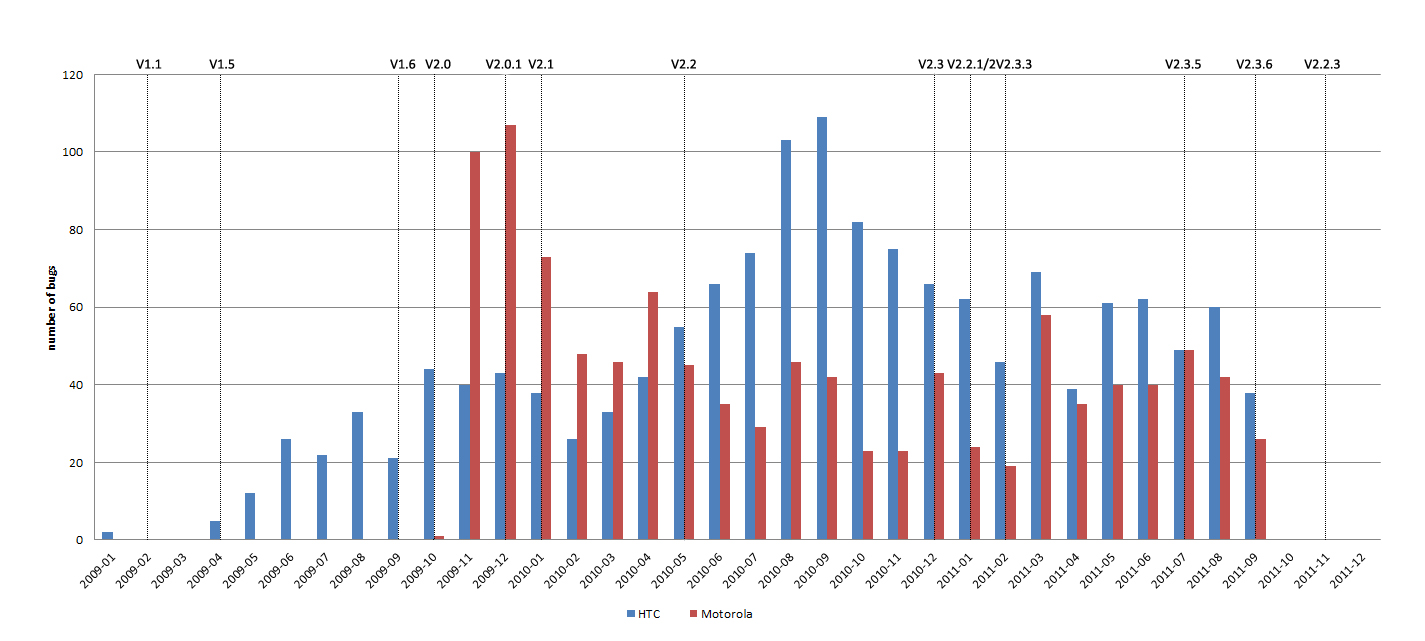
\includegraphics[width=1\textwidth]{bugovertime.png}
%\caption{Number of bugs with the major version of Android for HTC and Motorola}
%\end{figure*}



\section{Related Work}
\label{sec:relatedwork}
Topic models have been used to help understand software systems
features and link their artifacts together.
Marcus et al.~\cite{Marcus04aninformation} used Latent Semantic
Indexing (LSI) on both source code and user queries and then
identified the most relevant source code documents with similarity
measurements. 
Asuncion et al.~\cite{Asuncion:2010} applied a coherence measurement
on topics learned by LDA to model the quality of bug reports. 
Linstead et al.~\cite{Linstead:2009} performed LDA to generate
traceability links for artifacts in software projects automatically. 
Thomas et al.~\cite{Thomas:2011} studied
the evolution of topics within software projects.
While these studies used 
 LDA to extract topics,  we applied both Labeled-LDA and LDA to
obtain the topics. 
Unlike Labeled-LDA, LDA takes the number of topics as an input, but
the optimal number of topics can be subjective.
In our work, we first manually labeled the bug reports with multiple
labels and then employed
Labeled-LDA to associate topics and documents with the labels we
provided~\cite{labeledlda}. 
LDA cannot incorporate these manual labels during the learning process.
Our technique overcomes the disadvantages of these unsupervised
algorithms but at the expense of manual labeling.



\section{Methodology}
\label{sec:methodology}

Our methodology for investigating Android fragmentation starts by extracting
bug reports, labeling the bug reports and then applying
Labeled-LDA to the labeled bug reports.
Then 
 we calculate and visualize the average relevance of bug reports to each label
over time and compare them between two Android vendors,
HTC and Motorola, in order to look for fragmentation.
We also compare the performance of LDA topics versus
Labeled-LDA topics by comparing the 
the similarity of each pair of
topics from LDA and Labeled-LDA.

\subsection{Generating the data}

% 1. Extract data: We converted the XML dump of bug reports into SQL
% database. We extracted all the bug reports of HTC and Motorola from
% the SQL database using regular expressions,
% e.g. '%[^0-9a-z]HTC[^0-9a-z]%' and '%[^0-9a-z]motorola[^0-9a-z]%'. We
% also removed the declined and duplicated bug reports.

First, we
extract the Android bug reports and then find
the bug reports relevant to HTC and Motorola.  We parse and store the
Android bug reports provided by the MSR Mining
Challenge~\cite{MSRChallenge2012} as table in a SQL Server database.


Then we selected bug reports that identified themselves as being
relevant to HTC or Motorola if they mentioned HTC or Motorola in their
title text or their description text.
We then removed all the declined (unaccepted) and duplicate bug reports, leaving us
with 1503 HTC bug reports and 1058 Motorola bug reports.

\begin{table}[!t]
%\renewcommand{\arraystretch}{1.3}
% if using array.sty, it might be a good idea to tweak the value of
% \extrarowheight as needed to properly center the text within the cells
\caption{Manual labels applied to bug reports of HTC and Motorola.}
\label{selected1}
\centering
\begin{tabular}{|m{1.3cm}<{\centering}|m{.35\textwidth}<{\centering}|}
%|c||l|}
\hline
Vendor & Label\\
\hline
HTC & sms\/mms calling email contact video time network
    android\_market display browser bluetooth audio 
    notification image SIM\_card settings layout app 
    wifi google\_map keyboard calendar alarm language car 
    dialing USB touchscreen CPU gtalk voicedialing signal 
    google\_voice ringtone google\_navigation location font 
    google\_earth battery google\_translate twitter date VPN 
    picassa video\_call rSAP region screen\_shot download 
    IPV6 SD\_card storage 3G proxy compass calculator 
    synchronization  voicemail  voice\_recognition facebook flash 
    google\_latitude GPS camera youtube input search radio 
    system memory  upgrade  lock \\
\hline
Motorola & calling network settings gtalk calendar signal contact
      android\_market input camera image app wifi keyboard
      layout sms\//mms bluetooth display browser email
  alarm audio multimedia\_dock car SD\_card screen
  voicedialing battery upgrade dialing ringtone volume
  video time swype search exchange headset synchronization
  facebook google\_wave download youtube upload
  monkey flash VPN touchscreen vibrate CPU system
  notification text lock GPS calculator  USB\\
\hline
\end{tabular}
\end{table}


\subsection{Creating Labels and Training Annotators}

% 2. Where are the labels coming from: Before labeling all the bug
% reports, we studied the Android operating system to get the features
% of Android phones
% [http://en.wikipedia.org/wiki/Android_operating_system] and popular
% applications in Android Market
% [https://play.google.com/store/apps]. We also studied the hardware
% components of HTC and Motorola
% [http://en.wikipedia.org/wiki/Comparison_of_Android_devices]. The
% labels are based on these three aspects of Android phones.

To investigate hardware fragmentation from a feature-oriented
perspective we labeled the bug reports by their
relevant features. This allows us to find feature-relevant bug reports
for each manufacturer.
To ensure our feature-oriented labels would agree with actual
Android features we studied various descriptions~\footnote{Android Operating System summary:
\url{http://en.wikipedia.org/wiki/Android_operating_system};
Android Market: \url{https://play.google.com/store/apps};
Android Comparison:
\url{http://en.wikipedia.org/wiki/Comparison_of_Android_devices}
(retrieved March, 2012).}
 of Android's
operating system, popular apps, and the Android offerings of HTC and
Motorola.

%\subsection{Developing Labels}
%Multi-labeling}


% 3. Label the bug reports: Zhang and Fan labeled 248 HTC bug reports in
% 2009 separately and then compared the results by each bug to ensure
% the same interpretation of the labels from last step. Then Zhang and
% Fan labeled the rest of the bug reports separately.

%XXX we need a cite
Once we became familiar with the Android operating system and Android
ecosystem we needed to agree and train ourselves to consistently label
Android bug reports.
Following a grounded theory-like coding approach, similar to the
approach taken in by Hindle et al.~\cite{Hindle2011}, authors Zhang
and Fan selected a set of HTC 248 bug reports to label
separately. 

To label a bug report, our annotators (Zhang or Fan) read the bug
report text, both the title and the description, and  then based on their
personal interpretation they related that bug report to the relevant
features. This means that one bug report could receive multiple labels
if it is relevant to multiple identified features. Labels were created
as necessary: if a label regarding a feature did not already exist, it
was created.
Our labels 
consisted of the features, applications and hardware of Android phones
such as SMS/MMS, browser, Wi-Fi , GPS, screens and
keyboards.


To ensure consistency and agreement in labeling the authors trained
themselves in consistent labeling.
Each annotator, authors Zhang and Fan, separately labeled each of these 248 bug reports, 
with labels inspired by the previous research on Android
features. 
Upon completion of labeling, 
 Zhang and Fan compared the labels,
discussing label agreement and
disagreement in order to train themselves to consistently label bug
reports.
The topics of the labeled bug reports were also compared: each annotator's labeled data was used as input to
 Labeled-LDA which produced a set of topics.
The resulting test topics and their relevant bug reports were compared to ensure
that annotators had a 
consistent interpretation of the bug reports and their labels.



%First, two of us (Zhang and Fan) separately tag the HTC 248 bug
%reports in 2009 with the multiple labels. 
% Then we train each author’s labeled data with STMT. 
% By comparing each set of trained topics in the results and returning
% to the bug reports, we check to ensure the same interpretation of each
% bug when labeling. 
% Then we come up with the same labeling rules to process the data. 

\subsection{Labeling the HTC and Motorola Bug Reports}

Once the labeling rules were agreed upon each annotator (Zhang and Fan)
seperately labeled HTC and Motorola bug reports, taking over 60 man
hours of manual labeling effort.
%After this, we tag the rest of bug reports separately for both HTC and
%Motorola. 
%Using the previously stated labeling methodology, labels were created as necessary.
%When there is a bug report that cannot be tagged by the labels we
%already have, we would create a new label together based on our
%definition of labels, i.e. the functionalities and applications on an
%Android mobile phone or the components of the handsets. 
New labels were created as necessary: the label ``calculator'' was created because later in
Android's history there were 
several bug reports about the correctness of the
calculator's results. 
% So we added it to our labels. 
%The manual labeling took approximately 30 hours per person. 


1304 HTC and 985 Motorola bug reports were labeled with multiple
labels, leaving 199 and 73 bug reports that cannot be clearly labeled.
In total, there are 72 labels for HTC and 57 labels for Motorola.
Table \ref{selected1} lists all the manual labels from bug reports of HTC
and Motorola.

\subsection{Applying Labeled-LDA}


% 4. Apply Labeled-LDA:We applied the Labeled-LDA tool, Stanford Topic
% Modeling Toobox [http://nlp.stanford.edu/software/tmt/tmt-0.4/], to
% get the topic-document distribution on our labeled bug reports.

% 5. Calculate the average relevance of each label: The average
% relevance over time of each label is calculated for each vendor. For
% each label the average relevance in one month is the the sum of bug
% reports' relevance divided by the number of bug reports in this
% month. The plot of the average relevance of each label between HTC
% and Motorola is based on this calculation.


Once the bug reports were labeled we wanted to extract the topics
associated with the labels. First we had to process the bug reports 
in order to apply Labeled-LDA to the labeled bug reports. 
We converted the title and description of each bug report to lowercase,
split the text into tokens, and filtered out stop words (words that are less than 3 characters and
common English stop words such as ``all'', ``about'', ``the'',
``that'' and ``were'' ). Then produced word distributions from
these sets of bug-report derived words.

Separately, we applied Labeled-LDA to these processed HTC bug reports and Motrola bug reports.
%We then supplied Labelled-LDA with these word distributions of the bug reports.
Labeled-LDA produced the topics, word distributions, associated
with our labels, as well as a document-topic matrix which links our
labels (topics) to the bug reports from HTC and Motorola.
% in the each bug report corpus (HTC and
% Motorola).
%By applying Labeled-LDA to the bug reports of HTC and Motorola
%separately, we have the word distribution of each label and a matrix
%that provides the relationship between bug reports and the labels. 

Our topic analysis is based on these results. 
To visualize the association of a label (an extracted
Labeled-LDA topic) to bug reports over time,
%In order to investigate the trend of each label by time, 
we grouped
all the bug reports by month, from 2009 to 2011, based on their open
date for each of the two vendors. 
We then computed the average relevance values of bug
reports to this label in each month. 
The average relevance value of a label \begin{math} \l_i \end{math} in
month \begin{math} m_j \end{math} is the sum of all the relevance
values of this label over all bug reports in this month divided by the
number of bug reports in this month,
\begin{equation}
A(\l_i,m_j) = \frac{\sum_{\substack{k=1}}^{|m_j|}r(\l_i,d_k)}{|m_j|}
\label{equation1}
\end{equation}
where $r(\l_i,d_k)$ is the relevance value of label $\l_i$ to bug
report $d_k$, $|m_j|$ is the number of bug reports in this month. 
We generated a distribution of average relevance across three years of
Android history
each label, depicted in Figure \ref{commontopic}, Figure \ref{fixtopic},
Figure \ref{uniquehtc} and Figure \ref{uniquemoto}.


\subsection{Applying LDA}

% 6. Apply LDA: We applied LDA on HTC and Motorola bug reports. We
% tried a set of number of topics for both vendors and in each case we
% tried to label all the topics generated by LDA based on the manual
% labels.

% 7. Choose the number of topics in LDA: We chose the number of topics
% in LDA based the rules that the topics are distinct enough from each
% other, have no repetition and can be well interpreted by us (i.e. we
% can use the manual labels to tag them).


In order to compare the performance between LDA and Labeled-LDA and
 to see if Labeled-LDA is worth the manual labeling effort, 
we applied LDA to the same processed bug reports of HTC and Motorola
but without our manual labels. 

Applying LDA had one complication, LDA requires an input, $n$ that
determines the number of topics that LDA is supposed to extract. 
If $n$ is too large, the topics tend to repeat themselves and tend to
represent similar issues. 
If $n$ is too small, the topics tend to be cluttered and lack a
coherent focus.
This can be interpreted manually by reading the topics and evaluating
the top 10 or 20 words associated with a topic.
To choose the number of topics $n$, we ran LDA using multiple values
of $n$ ranging from 10 to 70, counting by 5,
on the bug reports of HTC. 
Three of the authors (Han, Zhang and Fan) evaluated the word distribution of each topic
together in each case of $n$. 
We determined if topics were distinct enough based on matching the
topics to labels we had created and used for Labeled-LDA. 
%Given
%our previous manual labels that were used by Labeled-LDA we tried to label these LDA topics
%with those labels. 
For a given $n$, if the labels did not repeat too much, and topics did not receive too
many labels, then we preferred that $n$ over others without these
characteristics.
The authors chose $n = 35$, as the topics generated by LDA with $n = 35$
were distinct from each other, had few repetitions and could be
interpreted well by the authors based on their own judgment.
Other researchers had some similar results
\cite{Thomas:2011,Hindle2011}. 

We applied the same process to the bug reports of Motorola and we chose
the number of topics to be $n = 30$. 
As described for the HTC bug reports, we also labeled each topics
generated by LDA with our manual labels.
Three of the authors annotated the topics together and it took two
hours in total to finish all the labeling work. 
Table \ref{seleted2} lists a few selected topics from LDA with manual labels.


\subsection{Comparing the Effort to Use LDA and Labeled-LDA}

% 8. Comparison of LDA and Labeled-LDA: For each pair of topics in LDA
% and Labeled-LDA, we computed the their similarity based on the
% topic-document distribution. That is the Jaccard similarity of the two
% sets. One is from LDA and the other one is from Labeled-LDA. Each set
% is the bug reports that have relevance to that label. We chose several
% thresholds on the relevance. That is if the relevance is under the
% threshold, this bug report is not related to that label. At last we
% chose threshold to be 0.2 the mean of the similarities is the
% biggest. 

In order to determine if LDA would generate similar results to
Labeled-LDA we had to compare the topics of each.
% Thus nce LDA and Labelled-LDA were applied to the bug reports of HTC and
% Motorola we had to compare the topics that were extracted.
Both LDA and Labeled-LDA produce matrices of
 the relationships between bug reports of two vendors and the
labels or topics.
Thus we wanted to know if the LDA extracted topics that we manually
labeled matched the Labeled-LDA topics that were labeled via our bug
report labeling. If the results were similar there would be little
point in applying Labeled-LDA in the future.

We determined topic similarity by comparing the sets of documents
relevant to a LDA topic and those relevant to a Labeled-LDA
topic. Because the LDA topic might be different from the Labeled-LDA
topic we did pair-wise similarity comparisons.

We applied the Jaccard similarity coefficient to compute the
similarity between each topic in LDA and each label in Labeled-LDA. 
That is, the Jaccard similarity coefficient between label A in LDA and
label B in Labeled-LDA is the ratio of the intersection of bug reports
related to label A and label B to the union of the bug reports related
to label A and label B,
\begin{equation}
sim(A,B) = \frac{\phi(A,d)\bigcap\phi(B,d)}{\phi(A,d)\bigcup\phi(B,d)}
\end{equation}
where the $\phi(A,d)$ is the set of bug reports that has relevance
values to label A and $d$ is a set of all the bug reports in each
vendor.

The topic-document matrix often contains noise and weak
relationships between topics and documents, thus it is necessary to
provide a threshold of document relevance to determine if a document
is relevant to a topic or not.
We used several thresholds (0.01, 0.05, 0.1, 0.2, 0.3, 0.4 and 0.5) on
the relevance value of a bug report to a topic in LDA when generating
the Jaccard similarity coefficients. 
We eventually chose $0.2$ as the similarities had the biggest mean
value. 
We plotted these pairwise tests (see Figure \ref{similarityhtc} and
Figure \ref{similaritymoto}) in order to explore the match between
LDA and Labeled-LDA.

Then we counted the number of bug reports which are related to labels
that are both shared by LDA and Labeled-LDA in HTC and Motorola. 
We applied the Chi-squared test on the two sets of distribution to
study if each of the two distributions match.



\begin{table}[!t]
\renewcommand{\arraystretch}{1.3}
% if using array.sty, it might be a good idea to tweak the value of
% \extrarowheight as needed to properly center the text within the cells
\caption{Selected topics from LDA with manual labels. Word lists are inferred by LDA.}
\label{seleted2}
\centering
\begin{tabular}{|c||c||l|}
\hline
Vendor & Label & Top 10 terms\\
\hline
HTC & sms\//mms &sms, message, text, sent, send, conversation, \\
            && received, reply, time, number \\ \cline{2-3}
  & email & Email, mail, gmail, app. Inbox, send, emails, \\
            &&message, client, read \\ \cline{2-3}
  & browser&browser, page, web, http, open, website, \\
            &&webview, click, url, load\\
\hline
Motorola & wifi &connect, xoom, hotspot, netbook, wifi, ssid, \\
           &&radio, connection, feature, model\\ \cline{2-3}
    &calendar& calendar, event, sync, appointment, date, google, \\
           &&time, droid, day, change \\ \cline{2-3}
    &contact & contact, google, number, address, list, facebook, \\
           &&droid, account, sync, separate \\
\hline
\end{tabular}
\end{table}


\section{Topic Mining and Analysis}
\label{sec:topicanalysis}

In order to investigate fragmentation within Android, we mined the bug
reports of Android and analyzed the topic analysis results both
quantitatively and qualitatively.
We started by exploring the distribution of the number of bug reports
over time for HTC and Motorola. Then we compared and discussed the
distribution of average relevance for each topic over time for both
vendors.


\begin{figure*}
\centering
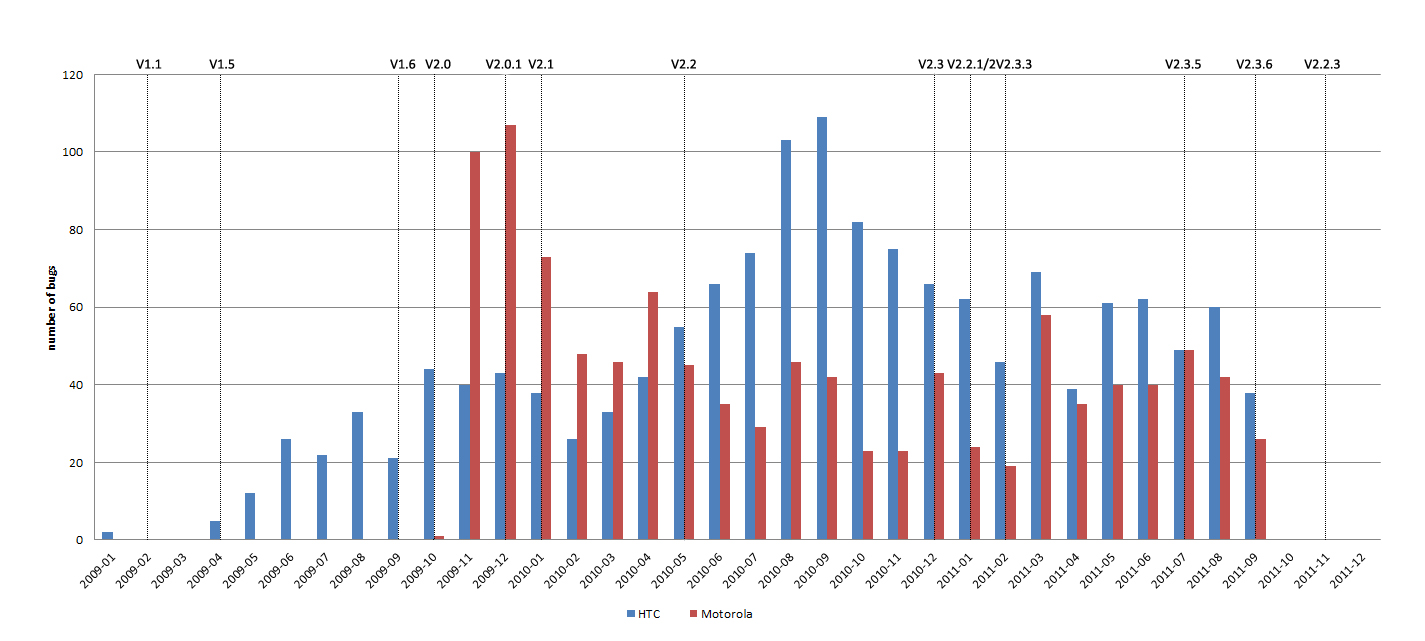
\includegraphics[width=1\textwidth]{bugovertime.png}
\caption{The number of bug reports over time for HTC and Motorola. The
  bottom
  horizontal axis is the months from January 2009 to December 2011. The top
  horizontal axis orders the Android versions by their released
  date. Vertical axis is the number of bug reports per month.}
\label{bugovertime}
\end{figure*}

\subsection{Overview of Bug Reports in HTC and Motorola}

We grouped the bug reports monthly based on their opened date and
counted the total number of bug reports in each month for two
vendors. 
Figure \ref{bugovertime} depicts a comparison of the number
of bug reports for each HTC and Motorola.


From Figure \ref{bugovertime}, we can observe that the first HTC bug
report was opened in January 2009, and the first Motorola bug report
was opened in October 2009.
According to the brief history of Android devices
survey~\cite{historyofandroid}, HTC released the first Android device
in Oct. 2008, while Motorola released its first device in Oct. 2009.
%The first bug reports of both vendors are in order of the first device
%released by them. 
There is a strong time correlation between the first
opened bug report and the first released Android device of both
vendors.
% In addition, Figure \ref{bugovertime} shows the peak of the number of
% bug reports for HTC happened in Sept. 2010, and for Motorola it
% happened in Dec. 2009. 


For HTC, out of 109 bug reports shown in that peak, 43 bug reports
were related with Android 2.1;
 and 50 bug reports were related with Android 2.2. 
By reading the bug reports, we found that the peak of HTC was caused
by the fact that many people upgraded Android from version 2.1 to
version 2.2,
and some features did not work well after upgrading, e.g, some users
could not send SMS messages anymore.
Thus Android upgrades for HTC tend to induce bug reports.


For Motorola,  95 out of 100 bug
reports in November 2009 were related to Android 2.0 on the Motorola Droid.
Among the 107 bug reports in December 2009, 54 bug reports were
associated with Android 2.0 and 53 bug reports were related to Android
2.0.1. 
We read many of these bug reports to find that most were related to this upgrade.
New features were also included in these ``upgrade bug reports''.
% Motorola released its first Android device, which is called Droid
% (different areas have different product model names, in Europe the
% model name is A853 or Milestone, in Latin America the model name is
% A854 or Motoroi). 
% It runs Android 2.0 with new features, such as touchscreen display,
% free turn-by-turn navigation from Google Maps, and sliding QWERTY
% keyboard. 
Other features that were prevalent in Motorola bug reports included
related to Google Maps and the sliding QWERTY keyboard. 
Much like HTC, Motorola bug reports were often caused by Android upgrades.


\subsection{Topics Analysis of HTC and Motorola}

In order to study the similarities and differences of bug reports in
Motorola and HTC we used topic analysis to pull out the trends of the
bug reports for each vendor.
Table \ref{selected1} shows that we extracted 72 topics for HTC and
57 topics for Motorola with Labeled-LDA.
Based on Equation \ref{equation1}, each topic has a distribution of
average relevance over time. 
We compared these distributions between vendors and categorized these
topics
into 
%XXX not sure if the distributions are shared
\textit{Common Topics}and \textit{Unique Topics}.
The \textit{Common Topics} represent the topics that are shared
between both vendors; common topics also tend to share 
similar distributions of the average relevance over
time.
The \textit{Unique Topics} represent those topics with significantly
different topic relevance over time (or topics that are completely
unique to either vendor).

% XXX TABLE TOPICSLIST IS DEFINED HERE
\begin{table*}[!htb]
%\renewcommand{\arraystretch}{1.3}
% if using array.sty, it might be a good idea to tweak the value of
% \extrarowheight as needed to properly center the text within the cells
\caption{Topics and associated Word List with Related Top 15 Terms}
\label{topicslist}
\centering
\begin{tabular}{|m{1.75cm}<{\centering}||m{7.33cm}<{\centering}||m{7.33cm}<{\centering}|}
\hline
%Topic Type & Label & HTC & Motorola\\ 
Label & HTC & Motorola\\ 
\hline
 sms\//mms &
message,  sms,  text,  thread,  time,  
sent,  desire,  contact,  new,  number,  
conversation,  send,  version,  app,  screen 
&
message,  text,  sms,  droid,  send, 
thread,  messaging,  sent,  user,  version, 
version,  person,  threads,  number,  http
\\ \hline

email &
email,  mail,  gmail,  app,  message,  
inbox,  messages,  client,  emails,  account,  
send,  interface,  thread,  time,  new 
&
email,  droid,  account,  gmail,  mail, 
server,  message,  user,  emails,  exchange, 
file,  version,  open,  device,  app
\\ \hline

calendar 
&
calendar,  event,  day,  events,  google,  
view,  2.2,  time,  month,  date,  
version,  reminder,  appointment,  edit,  running 
&
calendar,  event,  droid,  google,  appointment, 
events,  day,  field,  date,  appointments, 
 outlook,  milestone,  data,  app,  version
\\ \hline

contact
&
contact,  contacts,  number,  freed,  activity,  
displayed,  list,  group,  google,  numbers,  
starting,  desire,  user,  version,  field 
&
contact,  contacts,  droid,  number,  numbers, 
address,  version,  google,  menu,  correct, 
behavior,  different, list,  option,  gmail
\\ \hline

display
&
screen,  version,  desire,  behavior,  app,  
home,  number,  code,  final,  press,  
  sure,  user,  black,  new,  power 
&
droid,  screen,  button,  correct,  home, 
display,  behavior,  landscape,  2.1,  menu, 
bar,  xoom, device,  user,  status
\\ \hline


bluetooth
&
bluetooth, headset,  car,  connect,  device,  
connection,  version,  data,  app,  desire,  
desire,  2.2,  work,  connects,  behavior,  2.1 
&
bluetooth,  headset,  droid,  device, connected, 
connect,  devices,  calls,  car, issue, 
connection,  2.2,  car,  pair,  time
\\ \hline

synchronization
&
contacts,  account,  sync,  exchange,  contact,  
google,  ears,  device,  group,  server,  
Gmail,  policy,  new,  list,  display 
&
sync,  google,  account,  contacts,  device, 
contact,  group,  time,  exchange,  contacts, 
display,  groups,  list,  droid,  milestone
\\ \hline

settings
&
volume,  sound,  set,  pattern,  default,  
turn,  desire,  static,  control,  apps,  
change,  settings,  media,  dns,  screen 
&

settings,  device,  menu,  turn,  network, 
vpn,  honeycomb,  button,  xoom,  settings, 
behavior,  right,  wireless,  headset,  mode
\\ \hline


wifi
&
wifi,  access,  network,  connection,  connect,  
  router,  ssid,  desire,  http,  wi-fi,  
    device,  connected,  scan,  point,  app 
&
wifi,  xoom,  connect,  hotspot,  turn, 
 connection,  ssid,  radio,  error, signal, 
state,  user,  time,  feature, hotspots
\\ \hline

upgrade
&
update,  2.2,  file,  2.1,  google 
  version,  error,  upgrade,  froyo,  install,  
  work,  desire,  ota,  card,  ssl 
&
update,  droid,  2.1, 2.2,  home, 
http,  version,  user,  issue,  device, 
longer,  settings,  performance,  issues,  updated
\\ \hline

audio
&
music,  audio,  player,  file,  play,  
  2.2, sound,  version,  time,  playing,  
  playback,  app,  start,  reproduce,  mp3 
&
music,  droid,  player,  media,  audio, 
files,  volume,  play,  playing,  version, 
 app,  issue,  mode,  running,  genre,  sound,  user
\\ \hline

calling
&
number,  calls,  calling,  2.1,  receive,  
called,  button,  answer,  bluetooth,  desire,  
screen,  incoming,  works,  time,  magic 
&
droid,  calls,  number,  end,  button, 
answer,  incoming,  screen,  voice,  speaker, 
speaker,  2.2,  device,  place,  headphones
\\ \hline

android market
&
market,  app,  google,  account,  download,  
update,  application,  user,  device,  version,  
apps,  paid,  desire,  installed,  application 
&
market,  apps,  app,  device,  application, 
update,  open,  user,  version,  time, 
reporoduce,  download,  purchase,  google,  milestone
\\ \hline

image
&
image,  gallery,  picture,  matrix,  photo,  
null,  camera,  pictures,  version,  steps,  
2.2,  photos,  code,  display,  view 
&
image,  droid,  wallpaper,  gallery,  photo, 
picture,  device,  file,  select, video, 
 folder,  load,  live,  stock,  size,  screen
\\ \hline
\hline
language 
[HTC]
&
arabic,  desire,  language,  2.2,  letters,  
character,  translation,  character,  read,  support,  
sms,  write,  hebrew,  devices, 2.3 
&
NONE
\\ \hline
keyboard
[HTC]
&
keyboard,  input, text,  key,  version,  
number,  typing,  on-screen,  mode,  field,  
  landscape,  virtual,  keys,  type,  message 
&
keyboard,  droid,  keys, text,  press, 
space,  box,  open,  device,  key, 
app,  software,  2.0.1,  landscape
\\ \hline
\hline
GPS 
[Motorola]
& 
gps,  data, position,  location,  maps,  
google,  time, lock,  wrong,  icon,  turn,  
home,  latitude,  unit,  tag,  available 
&
maps,  gps,  google,  app,  droid, 
location,  application,  navigation,  map, device, 
traffic,  time,  upgrade,  turn,  route
\\ \hline
browser
[Motorola]
&
browser,  page,  text,  http,  open,  
server, verion,  desire,  client,  web,  
application, 2.1,  device,  button,  user 
&
browser,  droid,  page,  web,  http,  open, 
xoom,  html,  behavior,  running,  links, 
issue,  milestone,  3.1,  text
\\ \hline


\end{tabular}
\end{table*}

%%% Local Variables: 
%%% mode: latex
%%% TeX-master: t
%%% End: 


Table \ref{topicslist} depicts 
the top 18 most frequent labeled-topics of HTC and
Motorola.
Beside each topic we show the top 15 terms generated by Labeled-LDA for
each vendor. 
%As mentioned before, the label column in Table
%\ref{topicslist} represents the feature of Android.
%Please refer to the resarch features as potential labels 
%to have a better understanding of all the labels.

\begin{figure*}
\centering
%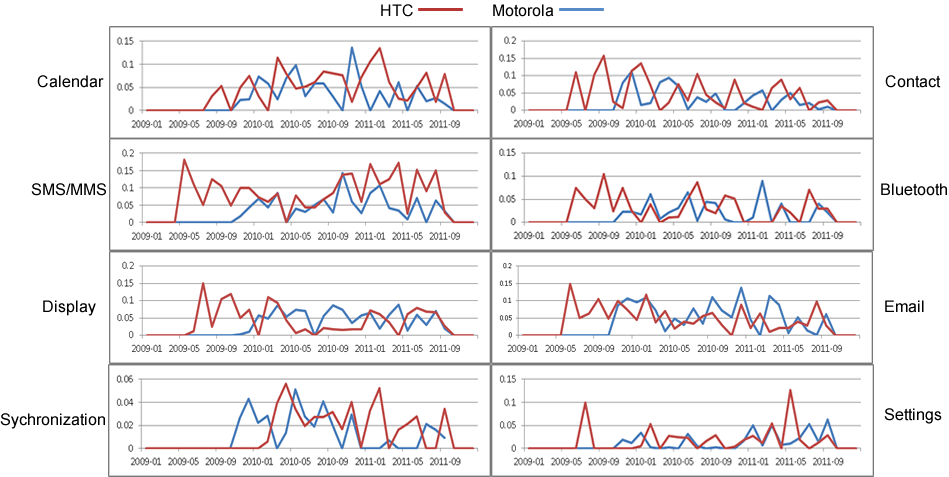
\includegraphics[width=1\textwidth]{commontopic.png}
%\begin{figure*}[htb]
%\centering
%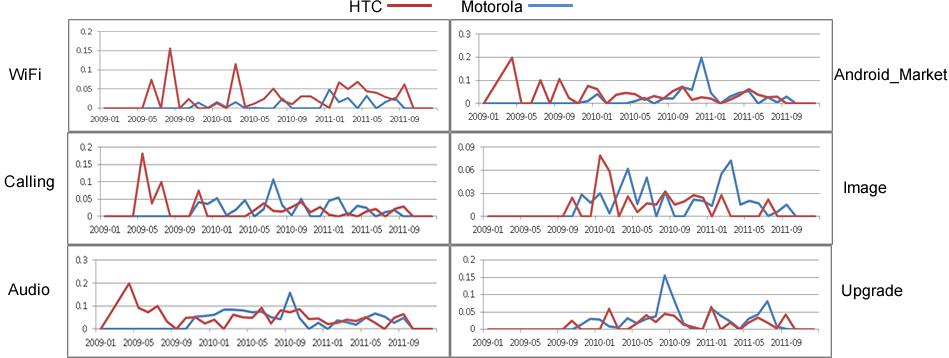
\includegraphics[width=1\textwidth]{fixtopic.png}
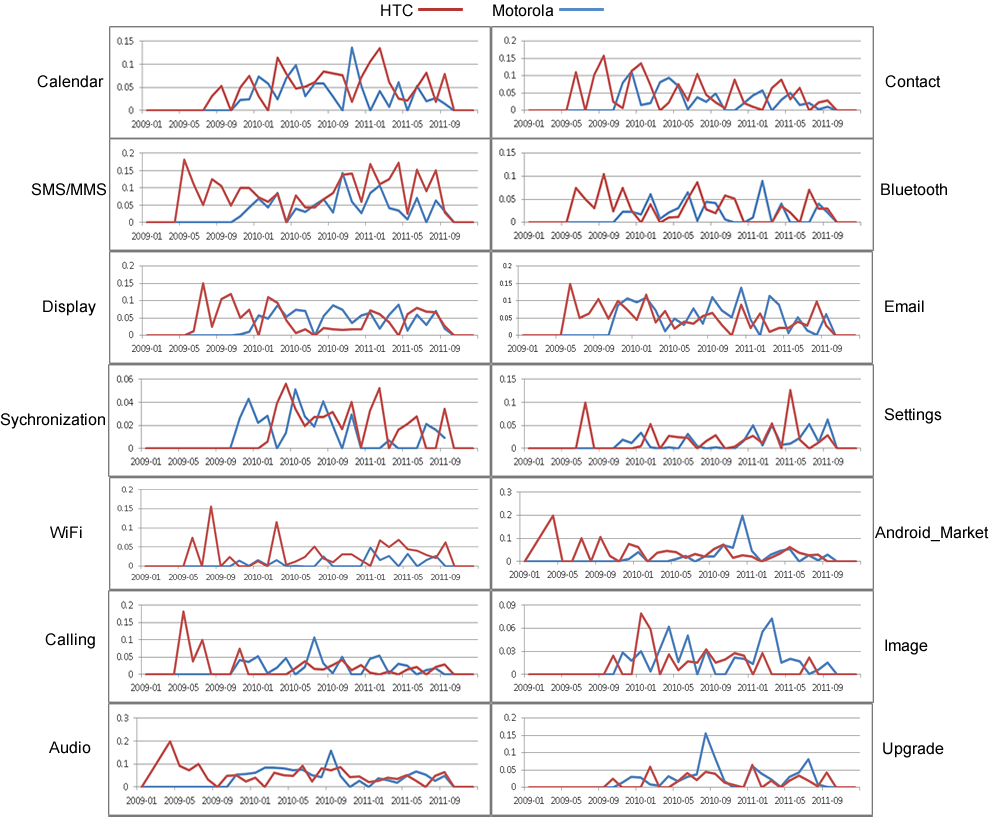
\includegraphics[width=1\textwidth]{combinedcommon.png}
\caption{Common Topics in HTC and Motorola. X axis is months from Jan. 2009 to Dec. 2011. Y axis is the average relevance of topics.}
\label{fixtopic}
%\end{figure*}
%\caption{Common Topics in HTC and Motorola. X axis is months from
%  Jan. 2009 to Dec. 2011. Y axis is the average relevance of topics.
%}
\label{commontopic}
\end{figure*}

\subsubsection{Common Topics}

There are fourteen \textit{Common Topics} shared by two vendors, shown
in 
Table \ref{topicslist}. 
Figure \ref{commontopic} depicts common topics between HTC and
Motorola. The top 8 topics are busy topics, whereas the bottom 6
topics peak and then flatten in interest over time.
% where HTC and 
% represent that the distribution of the average relevance of the topics
% have fluctuations all the time for both HTC and Motorola. In Figure
% \ref{fixtopic}, six topics represent that the distribution of the
% average relevance of topics turn to be flat over time after several
% fluctuations for HTC and Motorola.

The first 8 topics in Figure \ref{commontopic} share many identical
topic words between vendors.
Thus the bug reports use similar language between the vendors:
sms\//mms(\textit{text, thread, send}), calendar(\textit{event, day,
  google,appointment,time}), email(\textit{gmail, send, thread}),
contact (\textit{number, google,list}), display
(\textit{screen,button,behavior}), bluetooth (\textit{headset,connect,
  calling}), synchronize (\textit{contact, exchange, google}) and
settings(\textit{turn,network,mode}).
The \textit{Bluetooth} topic has a cross vendor peak 
with the release of both
 Android 2.1 and Android
2.2. 
% We did There
% is no obvious decreasing trends of bug reports with Android evolution.

The topics of one vendor tended to share vendor specific terms.
For instance, 5 of HTC's topics, \textit{sms\//mms, contact,
  display, bluetooth} and \textit{settings}, shared the term
``desire'', which refers to the HTC Desire phone.
%On the other hand, each vendor share the same terms in different
%topics. For HTC, five topics  share the same term
%``desire". This indicates that these topics happened frequently in
%``HTC Desire". 
% In the HTC topics \textit{Calendar} and \textit{bluetooth}
% share the same term ``2.2" which reveals that these two topics
% occurred frequently in Android 2.2. 
Motorola topics tend to share the term ``droid'' and the term ``xoom'', which refers to their
Motorola Droid and Motorola Xoom line of smartphones.
Motorola topics that mentioned ``Xoom'' included \textit{display,
  settings} and \textit{synchronize}.
Thus there is evidence that different product lines, faced different issues.
%For Motorola, seven topics except
%\textit{settings} share the same term ``droid" which stands these
%topics have high relevance with ``Motorola Droid". In addition,
%``xoom" shared by \textit{display} and \textit{settings} indicates
%that there are lots of bug reports related with these two topics in
%``Motorola Xoom". Furthermore, \textit{synchronize} associates with
% both ``xoom" and ``milestone" terms. This indicates bug reports
% related with \textit{synchronize} happened frequently in both Motorola
% Xoom and Motorola Milestone.

For Motorola vendor specific brand names tended to occur in the top
topic words of their common topics.
Six topics in Figure \ref{fixtopic} share many identical terms for
wifi (\textit{connection,ssid,network}), upgrade
(\textit{2.2,2.1,http}), and image(\textit{gallery,picture,photo}) in
HTC and Motorola. For example, bug reports releated with
\textit{upgrade} happened frequently in both vendors when people
upgraded Android from 2.1 to 2.2. It indicates Android 2.2 might have
incompatibility issue with the upgrading devices.  

% There are some special terms in these six topics for each
% vendor. Table \ref{topicslist} shows bug reports of HTC related with
% \textit{calling} happened frequently in Android 2.1, and some of them
% related with \textit{image} and \textit{audio} happened frequently in
% Android 2.2. Four out of six topics have correlation with ``HTC
% Desire". For Motorola, bug reports related to \textit{calling}
% happened frequently in Android 2.2. All of these topics have
% correlation with ``Motorola Droid" (``Motorola MileStone"). As a
% result, these six topics have a strong correlation with Android
% vendor's devices and some of topics have a strong correlation with
% Android versions.

In summary, both vendors share some same topics and terms associated
with these topics and also have the similar topics evolution over
time. HTC and Motorola topics tend to differ in terms of the
product-lines that appear in the topic words.
The ``HTC Desire", ``Motorola Droid", and  ``Motorola Xoom" are often
mentioned.
Both vendors share some \emph{common topics}, but even within these
topics and vendors it seems certain product-lines are affected by
different bugs. Thus this is evidence that there are portability
issues and fragmentation issues relevant to the shared \emph{common topics}
of vendors, and even across different vendor's smart-phone product
lines (Motorola Xoom and Droid correlated more with different topics).

% Thus this shows 
% These topics are common but there are platform specific issues that
% must be add
%  As a result, there might be
% portability issues in these topics for both vendors. Moreover, with
% Android evolution, some \textit{Common Topics} for both vendors have
% been correlated with the Android specific versions. As a result, there
% might be incompatibility problems in these Android features.

% \begin{figure*}[htb]
% \centering
% 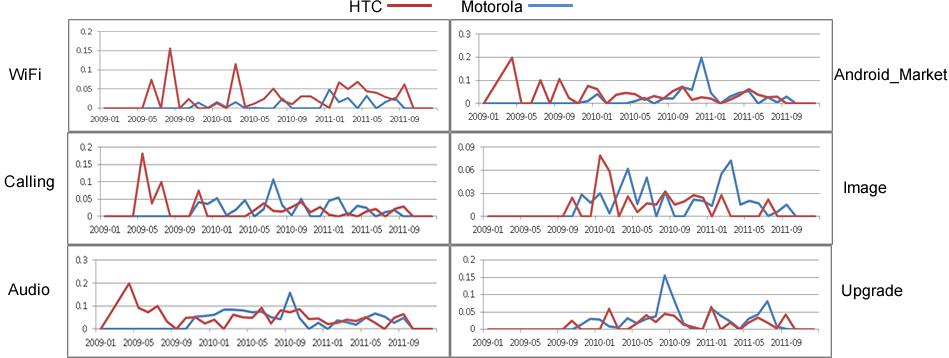
\includegraphics[width=1\textwidth]{fixtopic.png}
% \caption{Common Topics in HTC and Motorola. X axis is months from Jan. 2009 to Dec. 2011. Y axis is the average relevance of topics.}
% \label{fixtopic}
% \end{figure*}

\begin{figure*}
\centering
%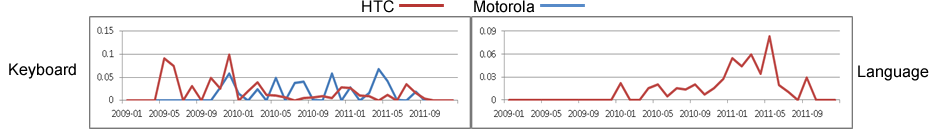
\includegraphics[width=1\textwidth]{uniquehtc.png}
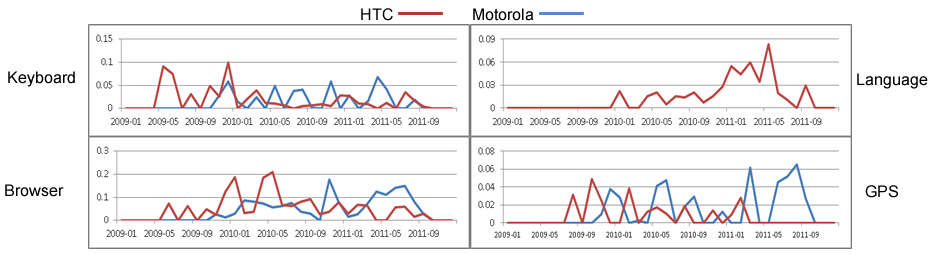
\includegraphics[width=1\textwidth]{combinedunique.png}
\caption{Unique Topics relevance in HTC (top) and Motorola (bottom). X axis is months from Jan. 2009 to Dec. 2011. Y axis is the average relevance of topics.}
\label{uniquehtc}
\label{uniquemoto}
\end{figure*}

% \begin{figure*}
% \centering
% 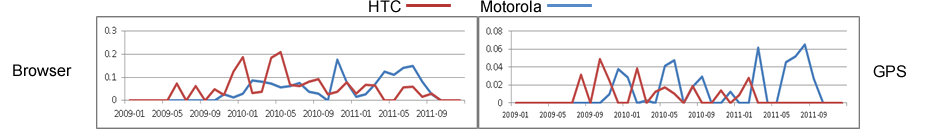
\includegraphics[width=1\textwidth]{uniquemoto.png}
% \caption{Unique Topics relevance in Motorola. X axis is months from Jan. 2009 to Dec. 2011. Y axis is the average relevance of topics.}
% \label{uniquemoto}
% \end{figure*}

\begin{figure*}
\centering
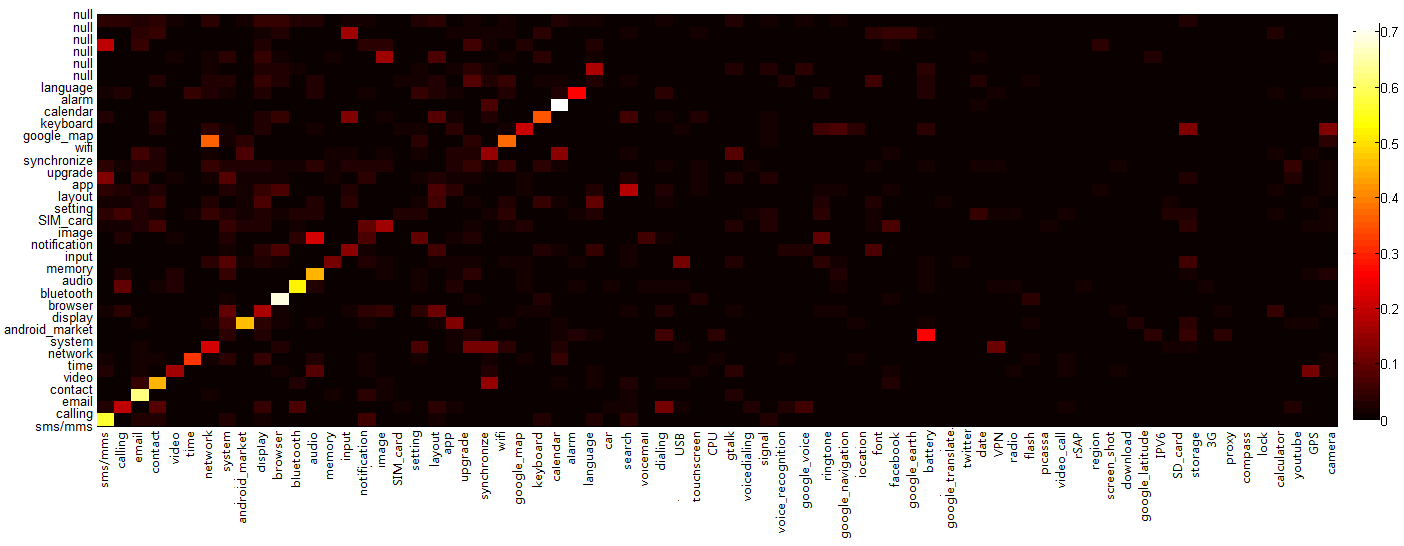
\includegraphics[width=1\textwidth]{htcsim.png}
\caption{Jaccard similarity of labels between LDA and Labeled-LDA in HTC. X axis is the labels in Labeled-LDA and Y axis is the labels of topics generated by LDA. The label ``null" in the Y axis means that topic cannot be labeled. The result is based on the HTC bug reports under the threshold of document relevance of 0.2. Brighter means higher Jaccard similarity.}
\label{similarityhtc}
\end{figure*}

\begin{figure*}
\centering
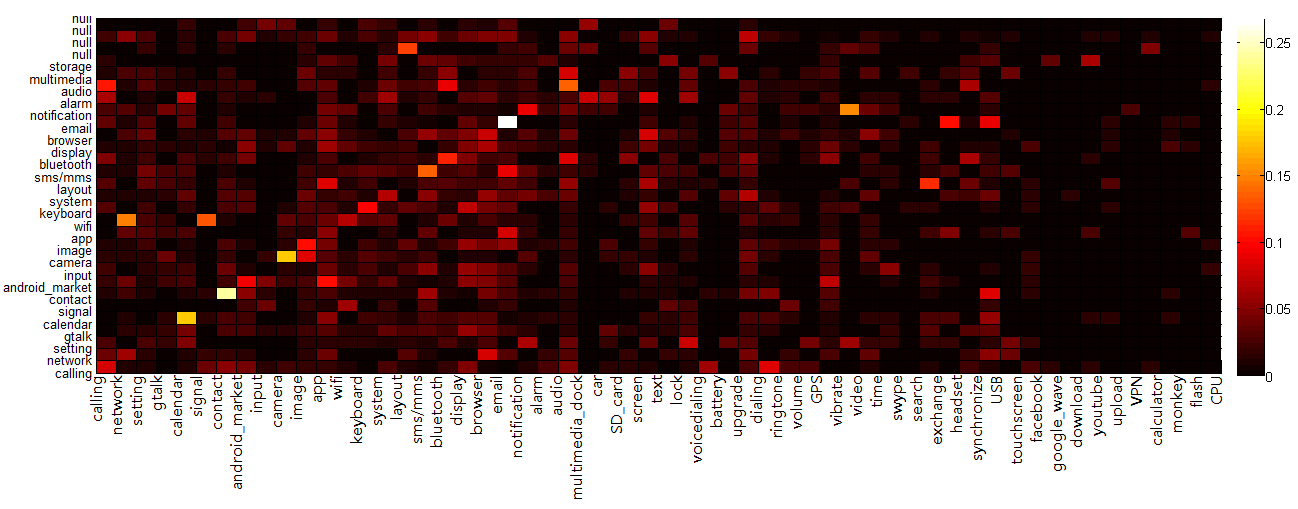
\includegraphics[width=1\textwidth]{motosim.png}
\caption{Jaccard similarity of labels between LDA and Labeled-LDA in Motorola. X axis is the labels in Labeled-LDA and Y axis is the labels of topics generated by LDA. The label ``null" in the Y axis means that topic cannot be labeled. The result is based on the Motorola bug reports under the threshold of document relevance of 0.2. Brighter means higher Jaccard similarity.}
\label{similaritymoto}
\end{figure*}


\subsubsection{Unique Topics}

Some topics are more unique to one vendor than the other.
%Both vendors not only have common topics, they also have unique
%topics. 
In Table \ref{topicslist} we present 2 unique HTC topics and 2 unique
Motorola topics. Figure \ref{uniquehtc} shows the distribution of the
average relevance of each of these unique topics for HTC and Motorola.


Topic \textit{language} (\textit{arabic, desire, language, 2.2, letters,
  characters, translation, character, read}) is an unique topic of
HTC. The associated terms indicate that bug reports related with
\textit{language}, and internationalization occurred frequently in
Android 2.2. 
This stems from
the fact that the feature of ``multiple keyboard languages" was a new
feature in Android 2.2. With this feature, multi-lingual users can add
multiple languages to the keyboard and switch between multiple
input languages~\cite{androidwebsite}. Most
HTC devices have no physical keyboards, so this new feature is 
frequently by HTC users. In contrast, Motorola's Android devices tend
to  have physical keyboards, which might explain the lack of activity
in the  Motorola bug reports.
Figure \ref{uniquehtc} shows that
HTC \textit{keyboard} relevance is steady, while \textit{keyboard} in
Motorola peaks and drops out. This behaviour suggests that hardware
and software configuration dictate the importance of the \emph{keyboard}
topic.
We did not notice internationalization or language issues in the
Motorola bug reports that we labeled, thus this issue seems more HTC
specific.


\textit{Browser} (\textit{browser, page, text, http, open, server}) is
an unique topics of Motorola. Table \ref{topicslist} shows that
Motorola's product lines,
s \textit{droid}, \textit{milestone} and \textit{xoom}, are relevant
to \textit{browser}.
Motorola's \textit{GPS} topic
(\textit{gps, data, position, location, maps, google, time, lock,
  wrong, icon, turn, home, latitude}), shown in Figure
\ref{uniquemoto},
starts slowly, peaks and drops off while HTC's GPS issues occur much
earlier and tend to fall off.
Motorola and HTC did not share the same GPS software at this
time. Thus GPS and browser are two topic where both vendor differ.

In summary, for both vendors, they have vendor specific topics which imply
there may be portability issues, and thus give rise to issues of
fragmentation, especially in terms internationalization, keyboards and
GPS support.

\section{Fragmentation Discussion}
\label{sec:fragmentation}
%What is feature evolution?


Many of our topics, bug reports, and peaks in activity are correlated
to Android releases such as versions 2.0, 2.1, and 2.2. It is
intuitive that new features and changes to the OS would induce bug
reports due to the difficulty in testing across all of these vendors
and product lines. The evidence we present indicates that
fragmentation might worsen the issues faced by users during an Android
OS version update.
Whether it is multiple versions of android that must be addressed or
the danger of Android updated, we witnessed both different and similar
behaviour within the bug reports of each vendor and their product-lines.


The variation in topic words in our \emph{common topics} tended to
relate to the distinct product lines of the vendors. Sometimes
different product lines were associated with different topics
indicating there might be fragmentation issues internal within the
product lines of a vendor.  The variation of hardware devices in each
vendor contribute to the bug topics about both Android features and
components of handsets. The \textit{Unique Topics} provide more
evidence that this might be the case.  Therefore, these portability
issue relevant to these bug topics leads us to conclude that \emph{there is}
some hardware fragmentation within Android.

When we refer to Android, we mean all the deployed Android versions
both from the community, vendors and carriers. We can see that Android
has a software fragmentation issue and it is evident in the issues
when updating, but we lacked a lot of necessary data to talk about the
conflicts caused by multiple supported versions of the same operating
system. Yet we can tell that the different hardware configurations,
especially keyboards, puts a different emphasis on relevant software
topics, such as software keyboards, within the bug repository per each
vendor.


\section{Comparing of LDA and Labeled-LDA}
\label{sec:comparinglda}

In this section we investigate if LDA and Labeled-LDA would generate
the similar results. This is an important issue because labelled-LDA
took at 60 times the amount of time it took to label the topics
extracted by plain LDA.

Figure \ref{similarityhtc} and Figure \ref{similaritymoto} depict the
pairwise Jaccard similarities of labels from LDA and Labeled-LDA. The
brighter spots mean the pair of labels have higher Jaccard
similarity. These two labels in LDA and Labeled-LDA are similar if
they share similar bug reports. The darker spots mean the pair of
labels have lower Jaccard similarity and share less bug reports in
common. 


%XXX could sub figure these.
\begin{figure}
\centering
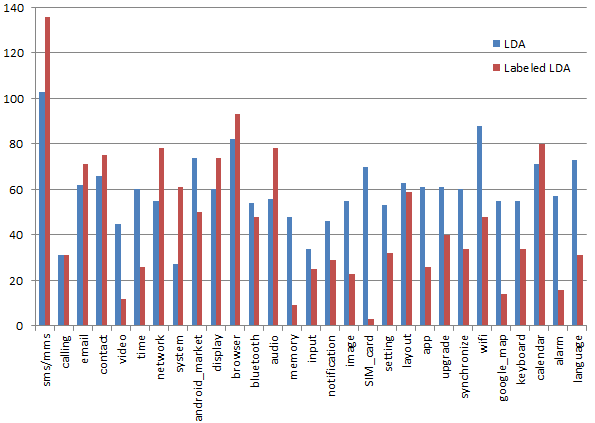
\includegraphics[width=0.5\textwidth]{htcldallda.png}
\caption{Comparison of number of bug reports related to the same labels from LDA and Labeled-LDA in HTC. The X axis is the same labels from LDA and Labeled-LDA and the Y axis is the number of bug reports.}
\label{bughtc}
\end{figure}

\begin{figure}
\centering
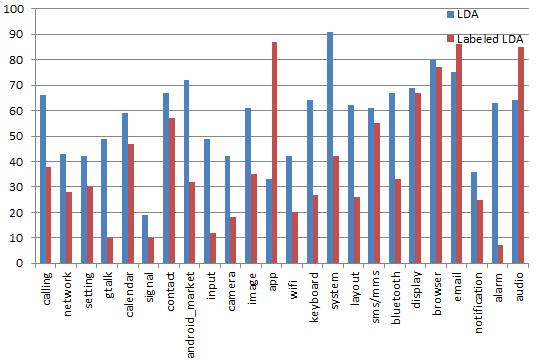
\includegraphics[width=0.5\textwidth]{motoldallda.png}
\caption{Comparison of number of bug reports related to the same labels from LDA and Labeled-LDA in Motorola. The X axis is the same labels from LDA and Labeled-LDA and the Y axis is the number of bug reports.}
\label{bugmoto}
\end{figure}


From these two Jaccard similarity plots (Figure \ref{similarityhtc}
and Figure \ref{similaritymoto}) of topics and labeled-topics between LDA and
Labeled-LDA, we can observe that most of the Jaccard similarity values
are quite small except a few diagonal ones, especially in HTC. This
observation is expected since most of the diagonal spots are the
Jaccard similarities between the same labels from LDA and
Labeled-LDA. However, even the mean similarities of the diagonal spots
are just about $0.2$ for HTC and $0.08$ for Motorola. The similarity plot
for Motorola has much more noise than the plot for HTC.
Thus the diagonals do match for Jaccard similarity but it is lower
than expected.

It became necessary to inspect the distributions of bug reports
associated with topics and labels more closely. 
Figure \ref{bughtc} shows the number of bug reports that are related to
the same labels in the bug reports of HTC and Figure \ref{bugmoto}
illustrates the number of bug reports that related to the same labels
in the bug reports of Motorola. The $ p $ values of the Chi-squared
%XXX validate this
test on the two sets of distribution are both close to zero ($p < 0.01$). Hence the
number of bug reports related to same labels in LDA and Labeled-LDA
are statistically significant quite different.


%Most of the same labels from LDA and Labeled-LDA have the comparable amount of bug reports. For example, the label ``calling'' from the HTC bug reports has exactly the same number of bugs related to for both results of LDA and Labeled-LDA. However, the similarity of these related bug reports in terms of this label ``calling'' is very low which means LDA and Labeled-LDA related quite different bug reports to this label. When doing this comparison, we cannot ignore the number of bugs that related to each label from both two techniques. That is, for one label, the ratio (the smaller number is divided by the bigger number so the ratio is always less or equal to one) of the number of bug reports related to this label predicted by LDA to that of Labeled-LDA would be the upper bound of the similarity value. From Figure \ref{bughtc} and Figure \ref{bugmoto} that the relation between topics and each bug report modeled by LDA is quite different from the results generated by Labeled-LDA.

%The similarity values for these labels in Figure \ref{similaritymoto} are quite low compared with the ratio. Only about ten labels in HTC have similarity values that are larger than half of the ratio. For Motorola, the similarity values are all very low compared with the upper bound of the similarity values.

We can conclude that only few of the bug reports in HTC and Motorola
are predicted by LDA and Labeled-LDA are related to the same
labels. In other words, the relation between topics and each bug
report modeled by LDA is quite different from the results generated by
Labeled-LDA. 
Thus LDA topics and Labeled-LDA topics are different, we found the
Labeled-LDA topics to be of better quality and matched better to our
goals; but we found that Labeled-LDA required up to and more than 60
times the effort that labeling LDA extracted topics required.




\section{Threats to validity}
\label{sec:threats}

\textit{Construct validity} – 
Our authors annotated 1000s of bug reports, their own biases could
have caused us to measure their biases rather than the features
relevant to the bug reports.
Also our automatic selection of Vendor-specific bug reports
might not accurately reflect the vendor-specific issues within the
bug repository.

% Our data originated from MSR Mining
% Challenge~\cite{MSRChallenge2012} and the dataset only ranges from
% 2009 to 2011. Furthermore we just took all the bug reports related to
% two vendors in this repository as the dataset to investigate. There
% may be other bug report repositories can be applied to increase the
% volume of our dataset.

\textit{Internal validity} – We argued the divergence of topics in
terms of relevance and keywords were indicators of fragmentation, thus
internal validity could be threatened by choices of parameters and labels.

% The explanations and theories we built
% are based on the actual distributions of all the average relevance of
% labels. The trends in the distributions are just manual observations
% instead of doing statistical analysis. We argue that the differences
% are distinct enough for us to just do observations. Besides, we might
% suffer from our bias when choosing the terms generated by Labeled-LDA
% for each label to do analysis.

\textit{External validity} – This study focused on one project,
Android, and two only vendors, HTC and Motorola, thus external
validity could be greatly improved by investigating other system such
as FreeBSD that face similar portability and fragmentation issues.

\textit{Reliability} – 
We carefully described our methodology and thus the methodology can be
repeated. Labels were applied using the judgment of two authors and
thus reliability suffers from the lack of repeatability in labeling --
although the training and correlation of labels that the authors
underwent should help bolster statistical reliability if someone were to
re-label the same data.
% The labels were from the studying features of
% Android system by two authors (Zhang and Fan). They cannot hide their
% previous expertise about Android system and handsets. The labels we
% come up with might suffer from the biased understanding of the aspects
% in Android system as well as mobile devices. Furthermore, when
% labeling the bug reports, two annotators followed the same protocol
% and used the same labels. However, they labeled all the bug reports
% separately. This might affect the labeling consistency in the dataset.


\section{Conclusions}
\label{sec:conclusions}

In this study we found evidence of fragmentation within Android by
comparing and contrasting the bug repository topics of 
two Android smartphone vendors: HTC and Motorola.
Based on Labeled-LDA topic analysis we found that even for shared \emph{common
topics} there was a divergence in topic keywords. We found that per vendor
different topics tended to be associated with their own different
products, providing even more evidence of vendor-specific fragmentation.
Thus our topic analysis provided evidence of hardware-based
fragmentation affecting the bugs being reported in the Android bug
repository.

We manually labeled 1000s of individual bug reports so that we could
apply Labeled-LDA and extract 
 feature-specific topics. We used our labeled bug reports to compare Labeled-LDA
and LDA, as LDA is unsupervised and far less effort to run than
Labeled-LDA.
We found that LDA (with manually labeled topics) and Labeled-LDA,
which needed labeled bug reports, produced some topics with some
cross-over but that the labeled-topics of Labeled-LDA were more
feature specific and more useful to our analysis. Yet the cost of
labeling bug-reports versus labeling LDA topics almost 2 orders of
magnitude greater in terms of man-hours.


%  to see if unsupervised LDA could produce similar topics to
% Labeled-LDA.
% We found that there was some crossover in topics but but not enough to be
% acceptable, thus we concluded that the topics of Labeled-LDA were
% different from topics of LDA, but Labeled-LDA required an order of magnitude
% more time to apply than  more effort in terms of
% time.
% %In this paper we studied Android bug reports for two vendors, HTC and
% %Motorola. Based on topic analysis using Labeled-LDA on a corpus of
% %manually tagged bug reports with multiple labels, we extracted the top
% %18 topics and categorized them into \textit{Common Topics} and
% %\textit{Unique Topics} for both vendors. Some of the \textit{Common
% %  Topics} show that there is no correlation between the features of
% %Android and Android evolution. In other words, there may be the
% %incompatibility problem existing to the specific features of
% %Android. Some of the \textit{Common Topics} show that some features
% %within the same vendors have portability issues across their multiple
% %devices. The \textit{Unique Topics} show that different vendor has
% %specific bug topics which imply there may be the portability problem
% %on the different vendors. Furthermore, we found that the manual
% % efforts of labeling all the bug reports would help us gain the better
% % topic models generated by Labeled-LDA after comparing LDA and
% % Labeled-LDA.

% For our future work, we will use the name of each hardware model as a
% label to do topic analysis while applying our methodology in order to
% discover the effects of different Android versions with respect to
% compatibility and stability. We will plan to investigate more vendors
% in order to reveal vendor specific bug topics.

%\subsubsection{Multi-labeling}
%Subsubsection text here.


%\begin{figure}[htb]
%\centering
%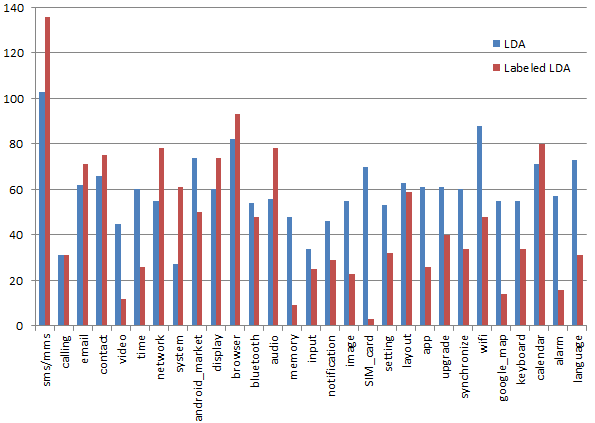
\includegraphics[width=0.4\textwidth]{htcldallda.png}
%\caption{Comparison of number of bug reports related to the same labels from LDA and Labeled-LDA in HTC. The X axis is the same labels from LDA and Labeled-LDA and the Y axis is the number of bug reports.}
%\end{figure}
%
%\begin{figure}[htb]
%\centering
%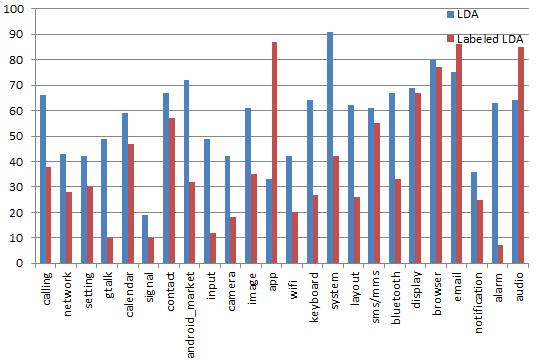
\includegraphics[width=0.4\textwidth]{motoldallda.png}
%\caption{Comparison of number of bug reports related to the same labels from LDA and Labeled-LDA in Motorola. The X axis is the same labels from LDA and Labeled-LDA and the Y axis is the number of bug reports.}
%\end{figure}
%
%\begin{figure}[htb]
%\centering
%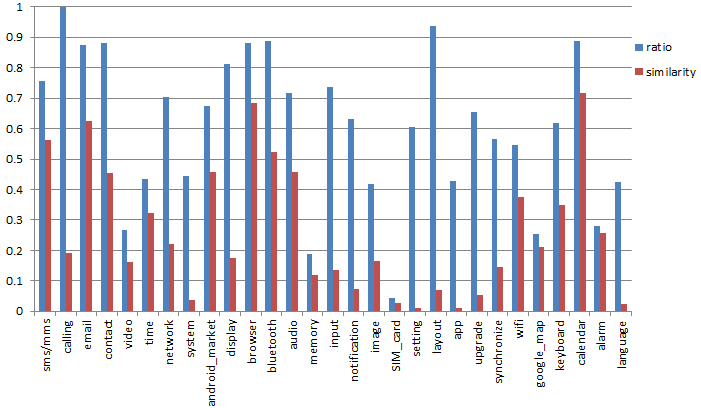
\includegraphics[width=0.4\textwidth]{htcratiosim.png}
%\caption{The comparison of ratio and similarity in HTC. The result of the smaller number of bug reports related to this label in LDA or Labeled-LDA divided by the larger one is the ratio of this label. The X axis is the same labels from LDA and Labeled-LDA.}
%\end{figure}
%
%\begin{figure}[htb]
%\centering
%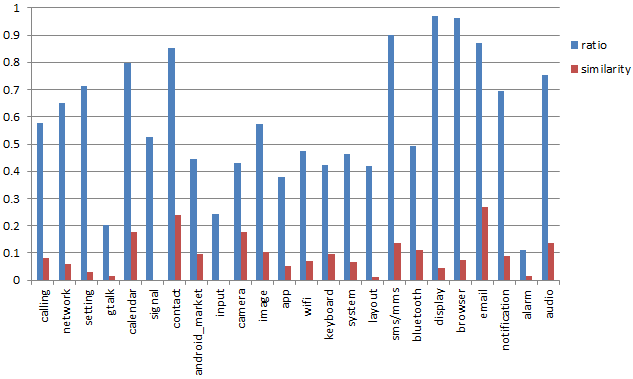
\includegraphics[width=0.4\textwidth]{motoratiosim.png}
%\caption{The comparison of ratio and similarity in Motorola. The result of the smaller number of bug reports related to this label in LDA or Labeled-LDA divided by the larger one is the ratio of this label. The X axis is the same labels from LDA and Labeled-LDA.}
%\end{figure}

% An example of a floating figure using the graphicx package.
% Note that \label must occur AFTER (or within) \caption.
% For figures, \caption should occur after the \includegraphics.
% Note that IEEEtran v1.7 and later has special internal code that
% is designed to preserve the operation of \label within \caption
% even when the captionsoff option is in effect. However, because
% of issues like this, it may be the safest practice to put all your
% \label just after \caption rather than within \caption{}.
%
% Reminder: the "draftcls" or "draftclsnofoot", not "draft", class
% option should be used if it is desired that the figures are to be
% displayed while in draft mode.
%
%\begin{figure}[!t]
%\centering
%\includegraphics[width=2.5in]{myfigure}
% where an .eps filename suffix will be assumed under latex, 
% and a .pdf suffix will be assumed for pdflatex; or what has been declared
% via \DeclareGraphicsExtensions.
%\caption{Simulation Results}
%\label{fig_sim}
%\end{figure}

% Note that IEEE typically puts floats only at the top, even when this
% results in a large percentage of a column being occupied by floats.


% An example of a double column floating figure using two subfigures.
% (The subfig.sty package must be loaded for this to work.)
% The subfigure \label commands are set within each subfloat command, the
% \label for the overall figure must come after \caption.
% \hfil must be used as a separator to get equal spacing.
% The subfigure.sty package works much the same way, except \subfigure is
% used instead of \subfloat.
%
%\begin{figure*}[!t]
%\centerline{\subfloat[Case I]\includegraphics[width=2.5in]{subfigcase1}%
%\label{fig_first_case}}
%\hfil
%\subfloat[Case II]{\includegraphics[width=2.5in]{subfigcase2}%
%\label{fig_second_case}}}
%\caption{Simulation results}
%\label{fig_sim}
%\end{figure*}
%
% Note that often IEEE papers with subfigures do not employ subfigure
% captions (using the optional argument to \subfloat), but instead will
% reference/describe all of them (a), (b), etc., within the main caption.


% An example of a floating table. Note that, for IEEE style tables, the 
% \caption command should come BEFORE the table. Table text will default to
% \footnotesize as IEEE normally uses this smaller font for tables.
% The \label must come after \caption as always.
%
%\begin{table}[!t]
%% increase table row spacing, adjust to taste
%\renewcommand{\arraystretch}{1.3}
%% if using array.sty, it might be a good idea to tweak the value of
%% \extrarowheight as needed to properly center the text within the cells
%\caption{An Example of a Table}
%\label{table_example}
%\centering
%% Some packages, such as MDW tools, offer better commands for making tables
%% than the plain LaTeX2e tabular which is used here.
%\begin{tabular}{|c||c|}
%\hline
%One & Two\\
%\hline
%Three & Four\\
%\hline
%\end{tabular}
%\end{table}


% Note that IEEE does not put floats in the very first column - or typically
% anywhere on the first page for that matter. Also, in-text middle ("here")
% positioning is not used. Most IEEE journals/conferences use top floats
% exclusively. Note that, LaTeX2e, unlike IEEE journals/conferences, places
% footnotes above bottom floats. This can be corrected via the \fnbelowfloat
% command of the stfloats package.


% use section* for acknowledgement
%\section*{Acknowledgment}


% trigger a \newpage just before the given reference
% number - used to balance the columns on the last page
% adjust value as needed - may need to be readjusted if
% the document is modified later
%\IEEEtriggeratref{8}
% The "triggered" command can be changed if desired:
%\IEEEtriggercmd{\enlargethispage{-5in}}

% Better way for balancing the last page:

%\balance

% references section

% can use a bibliography generated by BibTeX as a .bbl file
% BibTeX documentation can be easily obtained at:
% http://www.ctan.org/tex-archive/biblio/bibtex/contrib/doc/
% The IEEEtran BibTeX style support page is at:
% http://www.michaelshell.org/tex/ieeetran/bibtex/
%\bibliographystyle{IEEEtran}
% argument is your BibTeX string definitions and bibliography database(s)
%\bibliography{IEEEabrv,../bib/paper}
%
% <OR> manually copy in the resultant .bbl file
% set second argument of \begin to the number of references
% (used to reserve space for the reference number labels box)
%\begin{thebibliography}{1}

%XXX watch this
\vspace*{-0.5em}

\def\IEEEbibitemsep{0pt plus .5pt}
\small
\bibliographystyle{IEEEtran}
\bibliography{IEEEabrv,msrreference}
%\bibliography{msrreference}



\begin{comment}
%XXXX COMMENTED OUT XXXXX
%REPLACED BY AN INPUT \begin{table*}[!htb]
%\renewcommand{\arraystretch}{1.3}
% if using array.sty, it might be a good idea to tweak the value of
% \extrarowheight as needed to properly center the text within the cells
\caption{Topics and associated Word List with Related Top 15 Terms}
\label{topicslist}
\centering
\begin{tabular}{|m{1.75cm}<{\centering}||m{7.33cm}<{\centering}||m{7.33cm}<{\centering}|}
\hline
%Topic Type & Label & HTC & Motorola\\ 
Label & HTC & Motorola\\ 
\hline
 sms\//mms &
message,  sms,  text,  thread,  time,  
sent,  desire,  contact,  new,  number,  
conversation,  send,  version,  app,  screen 
&
message,  text,  sms,  droid,  send, 
thread,  messaging,  sent,  user,  version, 
version,  person,  threads,  number,  http
\\ \hline

email &
email,  mail,  gmail,  app,  message,  
inbox,  messages,  client,  emails,  account,  
send,  interface,  thread,  time,  new 
&
email,  droid,  account,  gmail,  mail, 
server,  message,  user,  emails,  exchange, 
file,  version,  open,  device,  app
\\ \hline

calendar 
&
calendar,  event,  day,  events,  google,  
view,  2.2,  time,  month,  date,  
version,  reminder,  appointment,  edit,  running 
&
calendar,  event,  droid,  google,  appointment, 
events,  day,  field,  date,  appointments, 
 outlook,  milestone,  data,  app,  version
\\ \hline

contact
&
contact,  contacts,  number,  freed,  activity,  
displayed,  list,  group,  google,  numbers,  
starting,  desire,  user,  version,  field 
&
contact,  contacts,  droid,  number,  numbers, 
address,  version,  google,  menu,  correct, 
behavior,  different, list,  option,  gmail
\\ \hline

display
&
screen,  version,  desire,  behavior,  app,  
home,  number,  code,  final,  press,  
  sure,  user,  black,  new,  power 
&
droid,  screen,  button,  correct,  home, 
display,  behavior,  landscape,  2.1,  menu, 
bar,  xoom, device,  user,  status
\\ \hline


bluetooth
&
bluetooth, headset,  car,  connect,  device,  
connection,  version,  data,  app,  desire,  
desire,  2.2,  work,  connects,  behavior,  2.1 
&
bluetooth,  headset,  droid,  device, connected, 
connect,  devices,  calls,  car, issue, 
connection,  2.2,  car,  pair,  time
\\ \hline

synchronization
&
contacts,  account,  sync,  exchange,  contact,  
google,  ears,  device,  group,  server,  
Gmail,  policy,  new,  list,  display 
&
sync,  google,  account,  contacts,  device, 
contact,  group,  time,  exchange,  contacts, 
display,  groups,  list,  droid,  milestone
\\ \hline

settings
&
volume,  sound,  set,  pattern,  default,  
turn,  desire,  static,  control,  apps,  
change,  settings,  media,  dns,  screen 
&

settings,  device,  menu,  turn,  network, 
vpn,  honeycomb,  button,  xoom,  settings, 
behavior,  right,  wireless,  headset,  mode
\\ \hline


wifi
&
wifi,  access,  network,  connection,  connect,  
  router,  ssid,  desire,  http,  wi-fi,  
    device,  connected,  scan,  point,  app 
&
wifi,  xoom,  connect,  hotspot,  turn, 
 connection,  ssid,  radio,  error, signal, 
state,  user,  time,  feature, hotspots
\\ \hline

upgrade
&
update,  2.2,  file,  2.1,  google 
  version,  error,  upgrade,  froyo,  install,  
  work,  desire,  ota,  card,  ssl 
&
update,  droid,  2.1, 2.2,  home, 
http,  version,  user,  issue,  device, 
longer,  settings,  performance,  issues,  updated
\\ \hline

audio
&
music,  audio,  player,  file,  play,  
  2.2, sound,  version,  time,  playing,  
  playback,  app,  start,  reproduce,  mp3 
&
music,  droid,  player,  media,  audio, 
files,  volume,  play,  playing,  version, 
 app,  issue,  mode,  running,  genre,  sound,  user
\\ \hline

calling
&
number,  calls,  calling,  2.1,  receive,  
called,  button,  answer,  bluetooth,  desire,  
screen,  incoming,  works,  time,  magic 
&
droid,  calls,  number,  end,  button, 
answer,  incoming,  screen,  voice,  speaker, 
speaker,  2.2,  device,  place,  headphones
\\ \hline

android market
&
market,  app,  google,  account,  download,  
update,  application,  user,  device,  version,  
apps,  paid,  desire,  installed,  application 
&
market,  apps,  app,  device,  application, 
update,  open,  user,  version,  time, 
reporoduce,  download,  purchase,  google,  milestone
\\ \hline

image
&
image,  gallery,  picture,  matrix,  photo,  
null,  camera,  pictures,  version,  steps,  
2.2,  photos,  code,  display,  view 
&
image,  droid,  wallpaper,  gallery,  photo, 
picture,  device,  file,  select, video, 
 folder,  load,  live,  stock,  size,  screen
\\ \hline
\hline
language 
[HTC]
&
arabic,  desire,  language,  2.2,  letters,  
character,  translation,  character,  read,  support,  
sms,  write,  hebrew,  devices, 2.3 
&
NONE
\\ \hline
keyboard
[HTC]
&
keyboard,  input, text,  key,  version,  
number,  typing,  on-screen,  mode,  field,  
  landscape,  virtual,  keys,  type,  message 
&
keyboard,  droid,  keys, text,  press, 
space,  box,  open,  device,  key, 
app,  software,  2.0.1,  landscape
\\ \hline
\hline
GPS 
[Motorola]
& 
gps,  data, position,  location,  maps,  
google,  time, lock,  wrong,  icon,  turn,  
home,  latitude,  unit,  tag,  available 
&
maps,  gps,  google,  app,  droid, 
location,  application,  navigation,  map, device, 
traffic,  time,  upgrade,  turn,  route
\\ \hline
browser
[Motorola]
&
browser,  page,  text,  http,  open,  
server, verion,  desire,  client,  web,  
application, 2.1,  device,  button,  user 
&
browser,  droid,  page,  web,  http,  open, 
xoom,  html,  behavior,  running,  links, 
issue,  milestone,  3.1,  text
\\ \hline


\end{tabular}
\end{table*}

%%% Local Variables: 
%%% mode: latex
%%% TeX-master: t
%%% End: 

\begin{table*}[!htb]
\renewcommand{\arraystretch}{1.3}
% if using array.sty, it might be a good idea to tweak the value of
% \extrarowheight as needed to properly center the text within the cells
\caption{Topics and associated Word List with Related Top 15 Terms}
\label{topicslist}
\centering
\begin{tabular}{|c||c||c||c|}
\hline
Topic Type & Label & HTC & Motorola\\ 
\hline
Common Topics & sms\//mms &message,	sms,	text, thread, time,  & message, text, sms, droid, send,	\\
&& sent, desire, contact, new, number, &	thread, messaging, sent,user, version,\\ 
&&conversation, send, version, app, screen &version, person, threads, number, http\\ \cline{2-4}

  & email & email, mail, gmail, app, message,   &email, droid, account,	gmail, mail, \\
&&inbox, messages,client,emails, account,  &server, message,user,emails, exchange, \\ 
&&send, interface, thread, time, new & file, version, open, device, app\\ \cline{2-4}
            
& calendar&calendar, event, day, events, google,  &calendar,	event, droid, google, appointment, \\
&&view, 2.2,time,month, date, &events, day, field, date, appointments, \\ 
&&version, reminder, appointment,  edit, running &outlook, milestone, data, app, version\\ \cline{2-4}
            
& contact & contact, contacts, number, freed, activity,  &contact, contacts, droid, number, numbers, \\
&&displayed, list, group, google, numbers,   &address, version, google, menu, correct, \\
&&starting,desire, user, version, field & behavior, different,list, option, gmail\\ \cline{2-4}
            
  & display&screen, version, desire,behavior, app, &droid, screen, button, correct, home, \\
&& home, number,code, final, press,  &display, behavior,  landscape, 2.1,  menu, \\
&&sure, user, black, new, power  &bar, xoom,device, user, status\\ \cline{2-4}
   
& bluetooth & bluetooth,headset, car, connect, device,  &bluetooth,	headset, droid, device,connected, \\
 &&connection, version, data, app, desire, & connect, devices, calls,car,issue,	\\
&&desire,	2.2, work, connects, behavior,2.1 & connection, 2.2, car,pair, time\\ \cline{2-4}
            
  & synchronization&contacts, account, sync, exchange, contact, &sync, google, account, contacts, device, \\
&&google, ears, device, group, server, &contact, group, time, exchange, contacts, \\
&&Gmail, policy, new, list, display&display, groups,  list,  droid, milestone\\ \cline{2-4}
            
  & settings&volume, sound,	set, pattern,  default,&settings, device, menu, turn,	network, \\
 && turn, desire, static, control, apps,&vpn, honeycomb, button, xoom,  settings, \\
  && change, settings, media, dns, screen &behavior,	right, wireless, headset, mode\\
\cline{2-4}

&wifi & wifi, access, network, connection, connect, &wifi, xoom, connect, hotspot, turn, \\
&&router, ssid, desire, http, wi-fi,&connection, ssid, radio, error,signal, \\

&&device, connected, scan, point, app &state, user, time, feature,hotspots\\ \cline{2-4}

&upgrade & update, 2.2, file, 2.1, google  & update, droid, 2.1,2.2, home, \\

 &&version, error, upgrade, froyo, install, & http, version, user, issue, device,\\           
 
 &&work, desire, ota, card, ssl & longer, settings, performance, issues, updated\\            \cline{2-4}
          
&audio& music, audio, player, file, play, &music, droid, player, media, audio,  \\

&&2.2,sound, version, time, playing, & files, volume, play, playing, version,\\

&&playback, app, start, reproduce, mp3 &app, issue, mode, running, genre, sound, user\\ \cline{2-4}
           
&calling& number, calls, calling, 2.1, receive, &droid, calls, number, end, button, \\
&& called, button, answer, bluetooth, desire,  &answer, incoming, screen, voice, speaker, \\ 

&& screen, incoming, works, time, magic & speaker, 2.2, device, place, headphones\\ \cline{2-4}
           
&android market& market, app, google, account, download, &market, apps, app, device, application,  \\

&&update, application, user, device, version, &update, open, user, version, time, \\ 
           
&&apps, paid, desire, installed, application & reporoduce, download, purchase, google, milestone\\ \cline{2-4}   
        
&image & image, gallery, picture, matrix, photo,  &image, droid, wallpaper, gallery, photo,\\
&&null, camera, pictures, version, steps,& picture, device,	file, select,video,\\

&&2.2, photos, code, display, view & folder, load, live, stock, size, screen\\

\hline
HTC Unique Topics & language 
&arabic, desire, language, 2.2, letters, & NONE\\

&&character, translation, character, read, support,& \\

&&sms, write, hebrew, devices,2.3 & \\ \cline{2-4}


& keyboard &keyboard, input,text, key, version,& keyboard, droid, keys,text, press, \\
&& number, typing, on-screen, mode, field, & space, box, open, device, key, \\
&&landscape, virtual, keys, type, message & app, software, 2.0.1, landscape \\
           
           
\hline
Motorola Unique Topics 
& GPS &gps, data, position, location, maps, & maps, gps, google, app, droid, \\

&&google, time,lock, wrong, icon, turn, & location, application, navigation, map,device, \\

&&home, latitude, unit, tag, available & traffic, time, upgrade, turn, route\\ \cline{2-4}

    &browser& browser, page, text, http, open, & browser, droid, page, web, http, open, \\
    &&server,verion, desire, client, web, & xoom, html, behavior, running, links, \\
&& application,2.1, device, button, user  & issue, milestone, 3.1,text \\
\hline
\end{tabular}
\end{table*}
\end{comment}


\end{document}
